\section{Teoria generale di limiti e colimiti}
Lo scopo di questa sezione è generalizzare le costruzioni date precedentemente a limiti e colimiti di forma diversa da prodotti, somme, equalizzatori e coequalizzatori. Dopo aver introdotto la nozione di cono e di cocono per un diagramma \(D \colon \ctJ \to\ctC\), il limite (risp., colimite) per \(D\) è l'oggetto terminale (risp., iniziale) della categoria dei coni (risp., coconi) per \(D\). In questo modo, si ottiene una definizione di limite e colimite che è del tutto generale, che si applica a qualsiasi tipo di diagramma, e che ritrova come esempi particolari tutti quelli fatti finora.

Ricordiamo che con \emph{diagramma} intendiamo un funtore \(D\colon \ctJ \fun \ctC\) da una categoria piccola \(\ctJ\) (detta \emph{categoria degli indici}) a una categoria \(\ctC\) (detta \emph{categoria ambiente}). La categoria indice è un modo per specificare la forma del diagramma, e dunque la forma del limite o colimite che vogliamo costruire. Ad esempio, se \(\ctJ\) è la doppia freccia generica, allora \(D\) è un diagramma di due frecce parallele, la categoria dei coni avrà per oggetti le frecce che equalizzano quella coppia, e il limite di \(D\) sarà il loro equalizzatore; se invece \(\ctJ\) è una categoria discreta con due oggetti, allora \(D\) è un diagramma di due oggetti, senza frecce tra loro, e il limite di \(D\) è un prodotto. E così via.
\begin{definition}[Categoria dei coni, categoria dei coconi]\label{def_cat_coni}
 \Todo{}
\end{definition}
\begin{definition}[Limite di un diagramma, colimite di un diagramma]\label{def_limite_colimite}
 \Todo{}
\end{definition}
\begin{remark}\label{rem_caratterizzazione_coni}
 Caratterizzazione equivalente della categoria dei coni e dei coconi per \(D\).
\end{remark}
\begin{remark}
 \Todo{A proposito del nome `cono' e `cocono'.}
\end{remark}
\begin{examples}\label{ex_cat_coni_coconi}
 Raccogliamo alcuni esempi di categorie di coni e di coconi per diagrammi noti e meno noti.

 Iniziamo coi prodotti di taglia arbitraria (piccola)
 \Todo{}

 \begin{itemize}
  \item Un oggetto terminale di \(\ctC\) è un cono terminale per il funtore vuoto \(\bang_\ctC \colon \ctInit\fun\ctC\). Dualmente, un	oggetto iniziale è un cocono iniziale per lo stesso funtore vuoto. (Si noti una certa autoreferenzialità: la categoria iniziale è il colimite del diagramma vuoto \(\bang_{\ctCat}\colon \ctInit \fun\ctCat\), e un oggetto iniziale (risp., terminale) in \(\ctC\) è un cocono (risp., un cono) per \(\colim(\bang_{\ctCat})\fun\ctC\). Questi diagrammi esistono, in un certo senso, su piani diversi.)
  \item Un equalizzatore è un cono terminale per un diagramma \(D \colon \genAArrow \fun\ctC\); dualmente, un coequalizzatore è un cocono iniziale dello stesso \(D\).  %(coppie nucleo e il quoziente di una relazione di equivalenza interna, fattorizzazione di un morfismo)
  \item Un equalizzatore \emph{riflessivo} è un cono terminale per \Todo{}
  \item Un prodotto fibrato è un cono terminale per un diagramma di dominio la cospanna generica di \ref{}; dualmente, una somma amalgamata è un cocono iniziale di un diagramma di dominio la spanna generica di \ref{}; strettamente parlando, nell'esempio precedente avremmo dovuto dire che un coequalizzatore è un cocono iniziale per \(D \colon (\genAArrow)^\op \fun\ctC\), ma la categoria \(\genAArrow\) è autoduale (si veda \ref{}).
  \item Un colimite filtrato è un cocono iniziale per un diagramma su una categoria filtrata nel senso di \ref{}; dualmente, un limite cofiltrato è un cono terminale per un diagramma su una categoria cofiltrata (equivalentemente, sull'opposta di una categoria filtrata). Un colimite in \(\kappa\)-catena è un cocono iniziale per un diagramma \(D \colon \kappa \fun \ctC\) come in \ref{}; dualmente un limite in \(\kappa\)-cocatena è un cono terminale per un diagramma	\(D \colon \kappa^\op \fun \ctC\).
  \item categorie puntate, nuclei e conuclei
  \item esempi e non esempi
 \end{itemize}
\end{examples}
\begin{example}\label{exa_gerarchia}\index{Gerarchia cumulativa}\index{Colimite!--- filtrato}
 \Todo{gerarchia cumulativa come colimite filtrato}
\end{example}
\begin{example}\label{ex_lim_padici}\index{Serie formale}\index{Limite cofiltrato|see {Colimite filtrato}}
 \Todo{Serie formali e \(p\)-adici come limite cofiltrato}
\end{example}
\begin{example}\label{ex_lim_frattali}\index{Frattale}\index{Coalgebra terminale}
 Alcuni frattali come coalgebre terminali
\end{example}
\begin{remark}\label{ex_colim_nat}
 Numeri naturali come colimite
\end{remark}
\subsection{Combinatoria dei co/limiti}
Per `combinatoria' dei co/limiti si intende l'insieme di tecniche per asserire che, assumendo alcune parti di un dato diagramma siano co/universali, anche altre parti lo sono. Il più semplice, e utile, risultato di questo tipo riguarda la possibilità di comporre, e cancellare, quadrati Cartesiani.
\begin{proposition}[Composizione di quadrati co/Cartesiani]\label{prop_composizione_quadrati_cartesiani}\index{Quadrato Cartesiano!composizione di ---}
%  \Todo{Incollamento di prodotti fibrati}
 Si consideri un diagramma della forma 
 \[\xymatrix{
  A \ar[r]^-f \ar[d]_-p\ar@{}[dr]|{(I)}& B\ar[r]^-g\ar@{}[dr]|{(II)} \ar[d]_q & C \ar[d]^r\\
  A'\ar[r]_-{f'} & B'\ar[r]_-{g'} & C'
 }\]
 e si chiami $(III)$ il quadrato 
 \[\xymatrix{
  A \ar[r]^-{g\cmp f}\ar[d]_p & C\ar[d]^r \\ 
  A' \ar[r]_-{g'\cmp f'}& C'
 }\]
 che risulta `componendo' nel senso ovvio i due quadrati, cioè componendo le frecce orizzontali. Allora, le seguenti condizioni sono equivalenti: 
 \begin{enumtag}{pb}
\item \label{pb_1} i quadrati $(I), (II)$ sono Cartesiani;
\item \label{pb_2} i quadrati $(II)$ e $(III)$ sono Cartesiani.
 \end{enumtag}
 Dualmente, le seguenti condizioni sono equivalenti: 
 \begin{enumtag}{po}
\item \label{po_1} i quadrati $(I), (II)$ sono coCartesiani;
\item \label{po_2} i quadrati $(I)$ e $(III)$ sono coCartesiani.
 \end{enumtag}
%  \Todo{Incollamento di somme amalgamate}
\end{proposition}
\begin{proof}
  Mostriamo l'equivalenza tra \ref{pb_1} e \ref{pb_2}, quella tra \ref{po_1} e \ref{po_2} segue per dualità.

  Assumendo che $(I), (II)$ siano Cartesiani, quello che va mostrato è che in un diagramma della forma
  \[\xymatrix{
    X \ar@/_1pc/[ddr]_v\ar@/^1pc/[drrr]^u\ar@{.>}[dr]|k & \\
  & A \ar[r]^-{f}\ar[d]_p &B\ar[d]_q\ar[r]^-g& C\ar[d]^r \\ 
  & A' \ar[r]_-{f'}&B'\ar[r]_-{g'}& C'
 }\]
  esiste un'unica freccia tratteggiata, che lo fa commutare in ogni parte. Del resto, la proprietà universale di $(\pull{B'}{C}{C'}, g,q)$ e la commutatività $r\cmp u = g'\cmp f'\cmp v$ implica che esista un'unica freccia $h : X \to B$ tale che $g\cmp h=u$ e $f'\cmp v = q\cmp h$. Ma ora, proprio per quest'ultima equazione e per la proprietà universale di $\pull{A'}{B}{B'}$, esiste un'unica $k : X \to A$ tale che $f\cmp k = h$ e $p\cmp k=v$; allora, quest'unica $k$ è anche tale che $g\cmp f\cmp k = g\cmp h = u$.

  Viceversa, se $(I)$ e $(III)$ sono Cartesiani, siamo nella situazione di questo diagramma:
  \[\xymatrix{
    X \ar@/_1pc/[ddr]_v\ar@/^1pc/[drr]^w\ar@{.>}[dr]|t & \\
  & A \ar[r]^-{f}\ar[d]_p &B\ar[d]_q\ar[r]^-g& C\ar[d]^r \\ 
  & A' \ar[r]_-{f'}&B'\ar[r]_-{g'}& C'
 }\]
  in cui ciascuna parte è commutativa. Dato che $(III)$ è Cartesiano, esiste un'unica $t : X \to A$ tale che $g\cmp w = g\cmp f \cmp t$ e $p\cmp t = v$; per concludere, manca di dimostrare che $q\cmp f\cmp t = q\cmp w$, e usare \ref{} ($f\cmp t = w$ è l'unica freccia di dominio $X$, tale che\dots); per vedere quest'ultima cosa, è sufficiente osservare che
  \[q\cmp f\cmp t = f'\cmp p\cmp t=f'\cmp v=q\cmp w.\]
  Questo conclude la dimostrazione.
\end{proof}
\begin{remark}
  Quanto dimostrato in \ref{prop_composizione_quadrati_cartesiani} è un risultato di `riduzione' tra prodotti fibrati innestati: assumendo che $B$ sia il prodotto fibrato $\pull {B'}C{C'}$, e che $A$ sia il prodotto fibrato $\pull{A'}{B}{B'}=\pull{A'}{(\pull {B'}C{C'})}{B'}$ allora 
  \[\pull{A'}{(\pull {B'}C{C'})}{B'} = \pull{A'}{(\pull {{\color{lightgray}B'}}C{C'})}{{\color{lightgray}B'}} \cong \pull{A'}C{C'}\]
  cosicché l'oggetto $B'$ può essere `semplificato'.
\end{remark}
\begin{remark}
 Si può mostrare, per induzione, un fatto più generale:
 \begin{quote}
  La composizione di \(n\)	quadrati Cartesiani come in
  % https://q.uiver.app/#q=WzAsMTIsWzUsMCwiQV8wIl0sWzQsMCwiQV8xIl0sWzMsMCwiQV8yIl0sWzIsMCwiXFxkb3RzIl0sWzEsMCwiQV97bi0xfSJdLFswLDAsIkFfbiJdLFs1LDEsIkFfMCJdLFs0LDEsIkFfMSJdLFszLDEsIkFfMiJdLFsyLDEsIlxcZG90cyJdLFsxLDEsIkFfe24tMX0iXSxbMCwxLCJBX24iXSxbNSwxMV0sWzUsNF0sWzQsM10sWzMsMl0sWzIsMV0sWzEsMF0sWzExLDEwXSxbMTAsOV0sWzksOF0sWzgsN10sWzcsNl0sWzAsNl0sWzEsN10sWzIsOF0sWzQsMTBdLFsxLDYsInFfMSIsMSx7InN0eWxlIjp7ImJvZHkiOnsibmFtZSI6Im5vbmUifSwiaGVhZCI6eyJuYW1lIjoibm9uZSJ9fX1dLFsyLDcsInFfMiIsMSx7InN0eWxlIjp7ImJvZHkiOnsibmFtZSI6Im5vbmUifSwiaGVhZCI6eyJuYW1lIjoibm9uZSJ9fX1dLFs0LDksInFfe24tMX0iLDEseyJzdHlsZSI6eyJib2R5Ijp7Im5hbWUiOiJub25lIn0sImhlYWQiOnsibmFtZSI6Im5vbmUifX19XSxbNSwxMCwicV9uIiwxLHsic3R5bGUiOnsiYm9keSI6eyJuYW1lIjoibm9uZSJ9LCJoZWFkIjp7Im5hbWUiOiJub25lIn19fV1d
  \[\begin{tikzcd}[ampersand replacement=\&,cramped]
    {A_n} \& {A_{n-1}} \& \dots \& {A_2} \& {A_1} \& {A_0} \\
    {B_n} \& {B_{n-1}} \& \dots \& {B_2} \& {B_1} \& {B_0}
    \arrow[from=1-1, to=1-2]
    \arrow[from=1-1, to=2-1]
    \arrow["{q_n}"{description}, draw=none, from=1-1, to=2-2]
    \arrow[from=1-2, to=1-3]
    \arrow[from=1-2, to=2-2]
    \arrow["{q_{n-1}}"{description}, draw=none, from=1-2, to=2-3]
    \arrow[from=1-3, to=1-4]
    \arrow[from=1-4, to=1-5]
    \arrow[from=1-4, to=2-4]
    \arrow["{q_2}"{description}, draw=none, from=1-4, to=2-5]
    \arrow[from=1-5, to=1-6]
    \arrow[from=1-5, to=2-5]
    \arrow["{q_1}"{description}, draw=none, from=1-5, to=2-6]
    \arrow[from=1-6, to=2-6]
    \arrow[from=2-1, to=2-2]
    \arrow[from=2-2, to=2-3]
    \arrow[from=2-3, to=2-4]
    \arrow[from=2-4, to=2-5]
    \arrow[from=2-5, to=2-6]
   \end{tikzcd}\]
  è ancora un	quadrato Cartesiano; se gli \(n-1\) quadrati \(q_1,\dots,q_{n-1}\) di destra sono Cartesiani, allora la composizione è Cartesiana se e solo se lo è il quadrato sinistro \(q_n\).
 \end{quote}
 (E ovviamente, uno duale per quadrati coCartesiani.) Ci si può domandare, ora, se è possibile generalizzare ulteriormente, per esempio `passando al limite' per \(n\to\infty\) avendo che la op-composizione transfinita (si veda \ref{})
 % https://q.uiver.app/#q=WzAsMTAsWzQsMCwiQV8wIl0sWzMsMCwiQV8xIl0sWzIsMCwiQV8yIl0sWzEsMCwiQV8zIl0sWzAsMCwiXFxkb3RzIl0sWzQsMSwiQV8wIl0sWzMsMSwiQV8xIl0sWzIsMSwiQV8yIl0sWzEsMSwiQV8zIl0sWzAsMSwiXFxkb3RzIl0sWzQsM10sWzMsMl0sWzIsMV0sWzEsMF0sWzksOF0sWzgsN10sWzcsNl0sWzYsNV0sWzAsNV0sWzEsNl0sWzIsN10sWzEsNSwicV8xIiwxLHsic3R5bGUiOnsiYm9keSI6eyJuYW1lIjoibm9uZSJ9LCJoZWFkIjp7Im5hbWUiOiJub25lIn19fV0sWzIsNiwicV8yIiwxLHsic3R5bGUiOnsiYm9keSI6eyJuYW1lIjoibm9uZSJ9LCJoZWFkIjp7Im5hbWUiOiJub25lIn19fV0sWzQsOCwicV97bi0xfSIsMSx7InN0eWxlIjp7ImJvZHkiOnsibmFtZSI6Im5vbmUifSwiaGVhZCI6eyJuYW1lIjoibm9uZSJ9fX1dLFszLDhdLFszLDcsInFfMyIsMSx7InN0eWxlIjp7ImJvZHkiOnsibmFtZSI6Im5vbmUifSwiaGVhZCI6eyJuYW1lIjoibm9uZSJ9fX1dXQ==
 \[\begin{tikzcd}[ampersand replacement=\&,cramped]
   \dots \& {A_3} \& {A_2} \& {A_1} \& {A_0} \\
   \dots \& {B_3} \& {B_2} \& {B_1} \& {B_0}
   \arrow[from=1-1, to=1-2]
   \arrow[from=1-2, to=1-3]
   \arrow[from=1-2, to=2-2]
   \arrow["{q_3}"{description}, draw=none, from=1-2, to=2-3]
   \arrow[from=1-3, to=1-4]
   \arrow[from=1-3, to=2-3]
   \arrow["{q_2}"{description}, draw=none, from=1-3, to=2-4]
   \arrow[from=1-4, to=1-5]
   \arrow[from=1-4, to=2-4]
   \arrow["{q_1}"{description}, draw=none, from=1-4, to=2-5]
   \arrow[from=1-5, to=2-5]
   \arrow[from=2-1, to=2-2]
   \arrow[from=2-2, to=2-3]
   \arrow[from=2-3, to=2-4]
   \arrow[from=2-4, to=2-5]
  \end{tikzcd}\]
 sia ancora un quadrato Cartesiano di forma
 \[\xymatrix{
  **[l]\lim A_n \mathrel{\rotatebox[origin=c]{180}{$\defeq$}} \hat A_\infty  \ar[r]^-{\pi_0} \ar[d] \ar@{}[dr]|{\hat q_\infty} & A_0 \ar[d] \\
  **[l]\lim B_n \mathrel{\rotatebox[origin=c]{180}{$\defeq$}} \hat B_\infty  \ar[r]_-{\pi_0} & B_0
}\]
 (E ovviamente, un eventuale risultato duale per quadrati coCartesiani.) Risponderemo a tempo debito.
\end{remark}
\begin{example}
 \Todo{Lemma del cubo}
\end{example}
\begin{example}
 Lemmi delle forme e degli animali (serpente, farfalla, salamandra, liocorno, teiera,	\dots)
\end{example}
\begin{example}
 \Todo{Quadrato magico di Vakil} Siano \(f_1,f_2 \colon X_1,X_2 \to Y\) e \(g \colon Y\to Z\) tre frecce di una categoria \(\ctC\); supponiamo che i prodotti fibrati \(\pull{X_1}{X_2}Y\) di \(f_1,f_2\), \(\pull {X_1}{X_2}Z\) di \(g\cmp f_1,g\cmp f_2\), e la coppia-nucleo \(\pull YYZ\) di \(g\), esistano tutte. Allora il quadrato colorato in rosso, ottenuto per funtorialità, è anch'esso un prodotto fibrato.
 % https://q.uiver.app/#q=WzAsMTEsWzAsMSwiWF8xXFx0aW1lc19ZIFhfMiJdLFsxLDAsIlhfMVxcdGltZXNfWiBYXzIiXSxbMiwxLCJYXzEiXSxbNCwwLCJYXzEiXSxbMCwzLCJYXzIiXSxbMiwzLCJZIl0sWzQsMiwiWiJdLFsxLDIsIlhfMiJdLFszLDIsIlkiXSxbNCwxLCJZIl0sWzMsMSwiWSBcXHRpbWVzX1ogWSJdLFs1LDYsImciLDJdLFsyLDMsIiIsMCx7ImxldmVsIjoyLCJzdHlsZSI6eyJoZWFkIjp7Im5hbWUiOiJub25lIn19fV0sWzQsNSwiZl8yIiwyXSxbMCw0XSxbMCwyXSxbMSwzXSxbMCwxLCJcXHB1bGx7WF8xfXtYXzJ9ZyIsMSx7ImNvbG91ciI6WzAsNjAsNjBdfV0sWzQsNywiIiwyLHsibGV2ZWwiOjIsInN0eWxlIjp7ImhlYWQiOnsibmFtZSI6Im5vbmUifX19XSxbMSw3XSxbNyw4LCJmXzIiLDAseyJsYWJlbF9wb3NpdGlvbiI6MjB9XSxbOCw2LCJnIl0sWzMsOSwiZl8xIl0sWzksNiwiZyJdLFsyLDVdLFsxMCw5XSxbMTAsOF0sWzEsMTAsIlxccHVsbHtmXzF9e2ZfMn1aIiwxLHsiY29sb3VyIjpbMCw2MCw2MF19XSxbMCw1LCIiLDAseyJjb2xvdXIiOlswLDYwLDYwXX1dLFs1LDEwLCJcXERlbHRhIiwwLHsiY29sb3VyIjpbMCw2MCw2MF19XSxbMTAsNiwiIiwwLHsic3R5bGUiOnsibmFtZSI6ImNvcm5lciJ9fV0sWzEsNiwiIiwwLHsic3R5bGUiOnsibmFtZSI6ImNvcm5lciJ9fV1d
 \[\begin{tikzcd}[ampersand replacement=\&,cramped]
   \& {X_1\times_Z X_2} \&\&\& {X_1} \\
   {X_1\times_Y X_2} \&\& {X_1} \& {Y \times_Z Y} \& Y \\
   \& {X_2} \&\& Y \& Z \\
   {X_2} \&\& Y
   \arrow[from=1-2, to=1-5]
   \arrow["{\pull{f_1}{f_2}Z}"{description}, draw={rgb,255:red,214;green,92;blue,92}, from=1-2, to=2-4]
   \arrow[from=1-2, to=3-2]
   \arrow["\lrcorner"{anchor=center, pos=0.125}, draw=none, from=1-2, to=3-5]
   \arrow["{f_1}", from=1-5, to=2-5]
   \arrow["{\pull{X_1}{X_2}g}"{description}, draw={rgb,255:red,214;green,92;blue,92}, from=2-1, to=1-2]
   \arrow[from=2-1, to=2-3]
   \arrow[from=2-1, to=4-1]
   \arrow[draw={rgb,255:red,214;green,92;blue,92}, from=2-1, to=4-3]
   \arrow[equals, from=2-3, to=1-5]
   \arrow[from=2-3, to=4-3]
   \arrow[from=2-4, to=2-5]
   \arrow[from=2-4, to=3-4]
   \arrow["\lrcorner"{anchor=center, pos=0.125}, draw=none, from=2-4, to=3-5]
   \arrow["g", from=2-5, to=3-5]
   \arrow["{f_2}"{pos=0.2}, from=3-2, to=3-4]
   \arrow["g", from=3-4, to=3-5]
   \arrow[equals, from=4-1, to=3-2]
   \arrow["{f_2}"', from=4-1, to=4-3]
   \arrow["\Delta", draw={rgb,255:red,214;green,92;blue,92}, from=4-3, to=2-4]
   \arrow["g"', from=4-3, to=3-5]
  \end{tikzcd}\]
\end{example}
\begin{proposition}
 Supponiamo di avere un cubo commutativo
 \[
  \xymatrix@R=.65em@C=.65em{
  A_0 \ar[rr] \ar[dd] \ar[dr] & & C_0 \ar[dd] \ar[dr] & \\
  & B_0 \ar[rr] \ar[dd] & & D_0 \ar[dd] \\
  A_1 \ar[rr] \ar[dr] & & C_1 \ar[dr] & \\
  & B_1 \ar[rr] & & D_1
  }
 \]
 in cui la faccia sinistra, la faccia destra e la faccia frontale sono Cartesiane. Allora la faccia posteriore è Cartesiana.
\end{proposition}
\begin{proof}
 \Todo{}
\end{proof}
\begin{proposition}
 Supponiamo di avere un cubo commutativo
 \[
  \xymatrix@R=.65em@C=.65em{
  A \ar[rr] \ar[dd] \ar[dr] & & C \ar[dd] \ar[dr] & \\
  & A' \ar[rr] \ar[dd] & & C' \ar[dd] \\
  B \ar[rr] \ar[dr] & & D \ar[dr] & \\
  & B' \ar[rr] & & D'
  }
 \]
 in cui le facce superiore e inferiore sono Cartesiane. Allora il seguente quadrato è Cartesiano,
 \[
  \begin{tikzcd}
   A \arrow[r] \arrow[d] & A' \arrow[d] \\
   B \times_D C \arrow[r] & B' \times_{D'} C'.
  \end{tikzcd}
 \]
\end{proposition}
\begin{proof}
 \Todo{}
\end{proof}
Entrambi questi risultati possono essere ottenuti come corollari del seguente fatto generale, che fa uso del calcolo dei sistemi di fattorizzazione (si veda \ref{}).
\begin{theorem}
 Sia \(\ctE\) una categoria che ammette prodotti fibrati. Se \(\ctB\) è la classe dei quadrati Cartesiani in \(\ctE\), e \(\ctA\) è la classe dei quadrati \(u \colon A \rightarrow B\) con \(u_1\) invertibile, allora la coppia \((\ctA, \ctB)\) è un sistema di fattorizzazione nella categoria \(\ctE^I\).
\end{theorem}
\subsection{Categorie piccolo-co/complete}
\begin{definition}[Categoria completa, \(\Phi\)-completa, piccolo-completa]\label{def_piccolo_complete}
 Diciamo che una categoria \(\ctC\) ammette limiti di forma \(\ctJ\) se ogni diagramma \(D \colon \ctJ \fun\ctC\) ammette un limite; più in generale, se \(\Phi\) è una sottoclasse degli oggetti di \(\ctCat\), diciamo che \(\ctC\) è \(\Phi\)-completa se per ogni \(\ctJ, D\colon\ctJ \fun\ctC\) esiste il limite di \(D\). In particolare, se \(\Phi=\ctCat_0\) è l'intera classe delle categorie piccole, la categoria \(\ctC\) si dice \emph{(piccolo-)completa}, oppure si dice che \(\ctC\) ammette tutti i limiti.

 Dualmente, diciamo che una categoria \(\ctC\) ammette colimiti di forma \(\ctJ\) se ogni diagramma \(D \colon \ctJ \fun\ctC\) ammette un colimite; più in generale, se \(\Phi\) è una sottoclasse degli oggetti di \(\ctCat\), diciamo che \(\ctC\) è \(\Phi\)-completa se per ogni \(\ctJ, D\colon\ctJ \fun\ctC\) esiste il colimite di \(D\). In particolare, se \(\Phi=\ctCat_0\) è l'intera classe delle categorie piccole, la categoria \(\ctC\) si dice \emph{(piccolo-)cocompleta}, oppure si dice che \(\ctC\) ammette tutti i colimiti.
 \Todo{}
\end{definition}
\begin{remark}
 Si noti che \(\Phi\) può essere una classe propria: ad esempio, \(\Phi\) può essere la collezione di tutte le categorie discrete, senza limite superiore di cardinalità, oppure la collezione di tutti gli ordinali, oppure di tutte le categorie connesse.
\end{remark}
Si è già osservato che la categoria	\(\ctSet\) di insiemi e funzioni ha prodotti (di qualsiasi cardinalità) ed equalizzatori di coppie di frecce. In effetti, è possibile sfruttare l'esistenza di questi soli limiti per dimostrare il seguente risultato generale (che, dualizzato, mostrerà l'enunciato duale).
\begin{example}\label{poset_cocompleti_se_somme}
 Un ordine guardato come categoria alla maniera di \ref{ord_sonocat} è una categoria piccolo-completa se e solo se ammette prodotti (cioè estremi inferiori) arbitrari; dualmente, è piccolo-cocompleta se e solo se ammette somme (cioè estremi superiori) arbitrari. Esempi di ordini piccolo-completi e piccolo-cocompleti sono: ogni algebra di Boole, ogni algebra di Heyting (e quindi in particolare gli insiemi potenza \(\pow S\) e gli insiemi degli aperti \(\tau_X\) di spazi topologici \((X,\tau_X)\)), \Todo{}
\end{example}
\begin{theorem}
 La categoria degli insiemi è piccolo-completa e piccolo-cocompleta.
\end{theorem}
\begin{proof}
 Per quanto riguarda la completezza,
 \Todo{dalle note di un'altra lezione:}
 \color{red}
 Let \(\ctJ\) be a small category and \(F \colon \ctJ\to\ctSet\) un diagramma. As in \ref{}, for every arrow \(f\) in \(\ctJ\), we denote \(\text{d}(f)\) the source and \(\text{c}(f)\) the target of \(f\); so, if \(f \colon J\to J'\), \(\text{d}(f)=J\), \(\text{c}(f)=J'\).

 We prove that the limit \(\lim F\) of \(F\) is precisely the equalizer of the pair of maps
 \[\xymatrix{
  \displaystyle\prod_{J\in\ctJ_0} FJ \ar@<.3em>[r]^-{\alpha^F}\ar@<-.3em>[r]_-{\beta^F}& \displaystyle\prod_{f\in\ctJ_1} F(\text{t}(f))
  }\]
 where
 \begin{itemize}
  \item \(\alpha^F(x_J\mid J\in\ctJ) = (x_{\text{t}(f)}\mid f\in\ctJ_1)\);
  \item \(\beta^F(x_J\mid J\in\ctJ) = (Ff(x_{\text{s}(f)})\mid f\in\ctJ_1)\);
 \end{itemize}
 This means two things: if \(\lim F\) exists, then it must be the equalizer of that pair; otoh, if that pair \((\alpha,\beta)\) has an equalizer, then such is the limit of \(F\).

 We have to prove that
 \begin{enumerate}
  \item There exists a cone
        \[\xymatrix{
         \lim F \ar[r]^-{\bar p} & \displaystyle\prod_{J\in\ctJ_0} FJ \ar@<.3em>[r]^-\alpha\ar@<-.3em>[r]_-\beta& \displaystyle\prod_{f\in\ctJ_1} F(\text{t}(f))
         }\]
        where \(e\) equalizes the pair \(\alpha,\beta\);
  \item such cone is terminal; this will mean two things:
        \begin{itemize}
         \item the universal property of \(\lim F\) entails the universal property of \(\mathsf{eq}(\alpha,\beta)\);
         \item the universal property of \(\mathsf{eq}(\alpha,\beta)\) entails the universal property of \(\lim F\).
        \end{itemize}
 \end{enumerate}
 Thus, there is a unique isomorphism \(\mathsf{eq}(\alpha,\beta)\cong \lim F\), which all in all exists because we have reduced the property of being a cone for \(F\) to the property of equalizing the pair \((\alpha,\beta)\). Since we know that \(\ctSet\) has products	and equalizers, we conclude that \(\lim F\) exists and thus that \(\ctSet\) is complete.

 Proving 1. is easy; if \((\lim F,p_J)\) exists, all projections \(p_J \colon \lim F\to FJ\) assemble into a unique map \(\bar p \colon \lim F \to \prod_J FJ\) (this is the universal property of \(\prod_J FJ\)). Note in passing that by the lemma above if \(\ctJ\) is a discrete category, \(\prod_{f\in\ctJ_1} F(\text{t}(f)) = \prod_{J\in\ctJ_0} FJ\), \(\alpha,\beta\) are invertible and thus \(\lim F\cong \prod_{J\in\ctJ_0} FJ\), as it should be.

 Now, \(\bar p \colon \lim F \to \prod_J FJ\) equalizes \((\alpha,\beta)\), because the components \(p_J\) form a cone: the triangle of sets and functions
 \[\xymatrix@R=5mm{
  & FJ \ar[dd]^{Ff}\\
  \lim F \ar[ur]^{p_J}\ar[dr]_{p_{J'}}& \\
  & FJ'
  }\]
 is commutative, whence the fact that for all \(\hat x\in\lim F\) and \(f \colon J\to J'\) in \(\ctJ_1\) one has
 \[
  \beta^F(\bar p(\hat x))= \big(Ff(p_{\text{s}(f)}(\hat x))\mid f\in\ctJ_1\big) =
  \big(p_{\text{t}(f)}(\hat x)\mid f\in\ctJ_1\big) = \alpha^F(\bar p(\hat x)).\]
 A similar argument for a general cone \((z \colon Z\to FJ\mid J\in\ctJ_0)\) proves that this is a cone for \(F\) if and only if it equalizes \((\alpha,\beta)\); thus, a cone for \(F\) must be a terminal cone wrt the property of equalizing \((\alpha,\beta)\); whence the conclusion.

 \color{black}
 Per quanto riguarda la cocompletezza,
 \Todo{}
\end{proof}
\begin{remark}
 \Todo{C'è una sezione comune per \(\alpha,\beta\)}
\end{remark}
Lo stesso ragionamento si applica ad altre categorie i cui oggetti sono insiemi, con una importante semplificazione nel caso di gruppi abeliani, spazi vettoriali, moduli su un anello, etc., dove possiamo semplificare l'espressione nel `teorema di struttura'; si veda \ref{}.
\begin{theorem}[Teorema di struttura sui limiti]\label{thm_struttura_limiti}
 Le condizioni seguenti sono equivalenti, per una categoria \(\ctC\).
 \begin{enumtag}{sl}
  \item\label{sl_1} piccolo-completezza nel senso di \ref{},
  \item\label{sl_2} avere tutti i prodotti e gli equalizzatori,
  \item\label{sl_3} avere tutti i prodotti e i prodotti fibrati,
  \item\label{sl_4} avere i limiti \(\kappa\)-cofiltrati per ogni \(\kappa\), i prodotti finiti e i prodotti fibrati, e
  \item\label{sl_5} avere i limiti \(\kappa\)-cofiltrati per ogni \(\kappa\), i prodotti fibrati e un oggetto terminale.
 \end{enumtag}
 Dualmente, le seguenti condizioni sono equivalenti:
 \begin{enumtag}{sc}
  \item\label{sc_1} piccolo-cocompletezza nel senso di \ref{},
  \item\label{sc_2} avere tutti i coprodotti e i coequalizzatori,
  \item\label{sc_3} avere tutti i coprodotti e le somme amalgamate,
  \item\label{sc_4} avere i colimiti \(\kappa\)-filtrati per ogni \(\kappa\), i coprodotti finiti e le somme amalgamate, e
  \item\label{sc_5} avere i colimiti \(\kappa\)-filtrati per ogni \(\kappa\), le somme amalgamate e un oggetto iniziale.
 \end{enumtag}
\end{theorem}
Valgono anche enunciati più deboli, che rimpiazzano \ref{sl_1} con la sola \(\lambda\)-completezza (cioè esistenza di tutti i limiti di diagrammi con dominio \(\lambda\)-piccolo); allora in \ref{sl_2}--\ref{sl_3} bastano i prodotti su famiglie \(\lambda\)-piccole, e in \ref{sl_4}--\ref{sl_5} `per ogni \(\kappa\)' diventa `ogni \(\kappa<\lambda\)'. Ovviamente, valgono (e saranno usati senza ulteriore menzione) risultati duali	a questi ultimi per la cocompletezza.
\begin{proof}
 La dimostrazione più comune della equivalenza tra tutte queste condizioni è quella che mostra l'equivalenza di \ref{sl_1} e \ref{sl_2}, e in effetti solo un'implicazione (l'altra è ovvia). Le altre procedono dimostrando che si possono esprimere i limiti di \ref{sl_3}, \ref{sl_4}, \ref{sl_5} l'uno in termini dell'altro.

 Si privilegia l'espressione di co/limiti generici in termini di co/equalizzatori di mappe tra co/prodotti perché la condizione \ref{sl_2} sostanzia nel modo migliore l'intuizione data in \ref{}, secondo cui un limite consta dell'oggetto `più grande in cui certe equazioni sono vere' e un colimite consta dell'oggetto `più piccolo in cui certe equazioni sono state imposte'.
\end{proof}
\begin{remark}
 Il risultato in \ref{} pone una domanda interessante: come si generalizza questo risultato? L'esistenza di esattamente \emph{quali} limiti è sufficiente all'esistenza di \emph{tutti gli altri} limiti? Cosa c'è di speciale nei prodotti e negli equalizzatori, e nei prodotti fibrati e oggetti terminali? La questione è affrontata in \cite{Albert1988}, e posta in questo modo, sebbene in un contesto ampiamente più generale:
 \Todo{}
\end{remark}
Per la parte che ci riguarda, riprenderemo la questione in \ref{}. Prima di procedere a dimostrare il teorema di struttura, un caso speciale di categoria di insiemi strutturati dove il risultato si adatta e si semplifica è la categoria dei gruppi abeliani (similmente si ragiona per moduli su un qualsiasi anello commutativo, e in particolare per gli spazi vettoriali).
\begin{remark}
 Nella categoria \(\ctAb\) dei gruppi abeliani, possiamo semplificare il teorema di struttura nell'enunciato che segue. Come è consuetudine, \(\ctJ_0\) e \(\ctJ_1\) indicano gli insiemi di oggetti e di frecce di \(\ctJ\), e \(c(u)\) e \(d(u)\) indicano rispettivamente il codominio e il dominio di una freccia \(u\in\ctJ_1\).
 \begin{quote}
  Sia \(D \colon \ctJ \fun \ctAb\) un diagramma. Allora, il limite di \(D\) è realizzato come il nucleo della mappa
  \[\xymatrix{
    \displaystyle\prod_{I\in\ctJ_0}DI \ar[r] & \displaystyle\prod_{u\in\ctJ_1} D(c(u))
   }\]
  che manda \(\big(x_I\mid I\in\ctJ\big)\) in \(\big(Du(x_I)-x_J \mid u \colon I \to J\big)\).

  Dualmente, il colimite di \(D\) è isomorfo al conucleo di una freccia
  \[\xymatrix{
    \displaystyle\bigoplus_{u\in\ctJ_1} D(d(u)) \ar[r] & \displaystyle\bigoplus_{I\in\ctJ_0}DI
   }\]
  tra somme dirette in \(\ctAb\), che applica la funzione \(\iota_J\cmp Du-\iota_I\) al generico elemento \((x_I\mid u\colon I\to J)\) del dominio (questi due elementi stanno in generale in sommandi diversi).

  (Dato che i prodotti e i coprodotti in questione possono essere infiniti, \(\bigoplus_I DI \subseteq \prod_I DI\) è un sottoggetto \emph{proprio}, si veda in tal senso \ref{})
 \end{quote}
 Per dimostrarlo, possiamo usare la semplice osservazione che dati due omomorfismi di gruppi abeliani \(f,g \colon A\to B\), l'equalizzatore di \((f,g)\) e il nucleo di \(g-f\) (e il nucleo di \(f-g\)) soddisfano tutti la stessa proprietà universale.
\end{remark}
\color{red}
\subsubsection{A propositio del teorema di esistenza dei colimiti}\label{sec_exist_colim}

\begin{color}{blue}
 Propongo la seguente formulazione, prima nel caso finito e poi nel caso generale, del teorema generale sull'esistenza dei (co)limiti.
 Il primo esempio prepara il teorema \ref{th_colim_piccoli}.
 L'esercizio conclusivo non c'entra niente con il teorema e può andare ovunque a condizione che si disponga delle nozioni di
 oggetto zero e di coprodotto.
\end{color}

\hfill

\noindent
Nella prossima proposizione vedremo due esempi, collegati fra di loro, di colimiti filtrati. Il secondo esempio sarà utilizzato nella
dimostrazione del teorema \ref{th_colim_piccoli}, teorema che permette di dedurre l'esistenza di tutti i colimiti piccoli dall'esistenza
di alcuni colimiti particolari.

\begin{proposition}\label{prop_coprod_colimfiltr}
 \hfill
 \begin{enumerate}
  \item Ogni insieme è il colimite dei suoi sottoinsiemi finiti. Inoltre tale colimite è filtrato perché l'insieme ordinato
        \(\ctP_f(I)\) dei sottoinsiemi finiti di un insieme \(I\) è chiaramente una categoria filtrata.
  \item Sia \(\ctC\) una categoria con i coprodotti finiti e sia \(\{X_i\}_{i \in I}\) una famiglia di oggetti di \(\ctC\) indicizzata da
        un insieme \(I\). Se il coprodotto della famiglia \(\{X_i\}_{i \in I}\) esiste, allora tale coprodotto è il colimite filtrato dei suoi sottocoprodotti
        finiti:
        \[\cop_{i \in I}X_i = \colim_{A \in {\cal P}_f(I)}\left(\cop_{a \in A}X_a\right)\]
        La stessa formula esprime il fatto che se in \(\ctC\) esistono i coprodotti finiti e i colimiti filtrati, allora in \(\ctC\) esistono tutti i coprodotti.
 \end{enumerate}
 Segnaliamo che i colimiti filtrati di questi esempi vengono chiamati anche colimiti diretti in quanto la categoria di base \(\ctP_f(I)\)
 utilizzata per definirli è un insieme ordinato diretto, cioè non vuoto e tale che ogni coppia di oggetti ha un maggiorante (vedi
 esempio \ref{esempio_2.5.42}).
\end{proposition}

\begin{proof} 1. La dimostrazione è facile e lasciata come esercizio per la lettrice. Alternativamente, il punto 1 si può trattare come
 caso particolare del punto 2, basta vedere un insieme \(I\) come il coprodotto di copie del singleton, una copia per ogni elemento di \(I\). \\
 2. Sia \(A \in \ctP_f(I)\), e sia
 \[s_A^a \colon X_a \to \cop_{a \in A}X_a\]
 il coprodotto con le iniezioni canoniche. Consideriamo il funtore \(S \colon \ctP_f(I) \fun \ctC\) che associa ad \(A \in \ctP_f(I)\) il coprodotto
 \(\cop_{a \in A}X_a\). A un'inclusione \(A \subseteq B\), il funtore \(S\) associa la freccia \(f^A_B\) definita dalla commutatività,
 per ogni \(a \in A\), del diagramma seguente:
 \[\xymatrix{\cop_{a \in A} X_a \ar[rr]^-{f^A_B} & & \cop_{b \in B} X_b \\
  & X_a \ar[lu]^{s^a_A} \ar[ru]_{s^a_B} }\]
 \(\bullet\) Se si assume l'esistenza del coprodotto \(\cop_{i \in I}X_i\) con le iniezioni \(s^i_I \colon X_i \to \cop_{i \in I}X_i\)
 allora tale coprodotto è anche il colimite del funtore \(S\).  Per ogni \(A \in \ctP_f(I)\), l'iniezione \(\sigma_A\) nel colimite è
 data dall'unica freccia che rende commutativo, per ogni \(a \in A\), il diagramma seguente:
 \[\xymatrix{\cop_{a \in A} X_a \ar[rr]^-{\sigma_A} & & \cop_{i \in I} X_i \\
  & X_a \ar[lu]^{s^a_A} \ar[ru]_{s^a_I} }\]
 \(\bullet\) Viceversa, se si assume l'esistenza del colimite del funtore \(S\) con iniezioni canoniche
 \[\sigma_A \colon \cop_{a \in A}X_a \to \colim_{A \in \ctP_f(I)}(\cop_{a \in A}X_a)\]
 allora tale colimite fornisce il coprodotto \(\cop_{i \in I}X_i\). Come iniezione nel coprodotto si prende, per ogni \(i \in I\), la freccia
 \[\sigma_{\{i\}} \colon X_i \to \colim_{A \in \ctP_f(I)}(\cop_{a \in A}X_a)\]
 Segnaliamo solo che per verificare la condizione di unicità nella proprietà universale del coprodotto è essenziale utilizzare la
 naturalità della famiglia \(\{\sigma_A \mid A \in \ctP_f(I)\}\). Lasciamo a chi legge il resto della verifica.
\end{proof}

\begin{theorem}\label{th_colim_fin}
 Sia \(\ctA\) una categoria. Le condizioni seguenti sono equivalenti:
 \begin{enumerate}
  \item \(\ctA\) ha i colimiti finiti.
  \item \(\ctA\) ha i coprodotti finiti e i coequalizzatori riflessivi.
 \end{enumerate}
\end{theorem}

\begin{proof}
 \begin{color}{blue}È la costruzione usuale, ma si osserva che la coppia di frecce parallele di cui si prende il
  coequalizzatore è un grafo riflessivo in \(\ctA\). \end{color}
\end{proof}

\begin{theorem}\label{th_colim_piccoli}
 Sia \(\ctA\) una categoria. Le condizioni seguenti sono equivalenti:
 \begin{enumerate}
  \item \(\ctA\) ha i colimiti piccoli.
  \item \(\ctA\) ha i colimiti finiti e i colimiti filtrati.
  \item \(\ctA\) ha i coprodotti finiti, i coequalizzatori riflessivi e i colimiti filtrati.
  \item \(\ctA\) ha i coprodotti finiti e i colimiti setaccianti.
  \item \(\ctA\) ha i coprodotti e i coequalizzatori riflessivi.
 \end{enumerate}
\end{theorem}

\begin{proof}
 \begin{color}{blue} Piuttosto che cercare la dimostrazione più rapida possibile, qua mi sembrerebbe
  interessante mettere in evidenza gli argomenti interessanti delle varie implicazioni.\end{color} \\
 \(2 \Rightarrow 1 \colon\) ogni colimite è il colimite del diagramma filtrato dei suoi sotto-colimiti finiti. \\
 \(2 \Leftrightarrow 3 \colon\) basta applicare il teorema \ref{th_colim_fin}.\\
 \(4 \Rightarrow 3 \colon\) i colimiti filtrati e i coequalizzatori riflessivi sono colimiti setaccianti. \\
 \(3 \Rightarrow 5 \colon\) ogni coprodotto è il colimite del diagramma filtrato dei sotto-coprodotti finiti. \\
 \(5 \Rightarrow 1 \colon\) si adatta in modo ovvio la costruzione fatta nella prova del teorema \ref{th_colim_fin}. \\
 Se si aggiunge che la condizione 1 implica ovviamente ognuna delle altre condizioni, la prova è completa.
\end{proof}

\begin{exercise}\label{exer_copr_retr}
 In questo esercizio ritroviamo una situazione ben nota nel caso dei monoidi, dei gruppi (abeliani o no), dei moduli
 su un anello, degli anelli senza unità. Sia \(\ctC\) una categoria con oggetto zero. Sia \(\{X_i\}_{i \in I}\) una famiglia
 di oggetti di \(\ctC\) e sia \(X = \cop_{i \in I}X_i\) il loro coprodotto. Ogni oggetto \(X_i\) è un retratto di \(X\).
\end{exercise}

La prossima proprietà si può esprimere dicendo che limiti e
colimiti nelle categorie di funtori si calcolano ``punto a punto''. Nelle proposizioni \ref{prop_lim_puntuali} e \ref{prop_fubini} e
nell'osservazione \ref{rem_fubini} trattiamo solo il caso dei limiti perché tutto si dualizza in modo ovvio. In particolare, nei
corollari \ref{cor_fun_cat_compl} e \ref{cor_lim_cat_pref} diamo per acquisita la duale della proposizione \ref{prop_lim_puntuali}.

\begin{proposition}\label{prop_lim_puntuali}
 Siano \(\ctB,\ctC,\ctD\) tre categorie, con \(\ctC\) e \(\ctD\) piccole. Consideriamo un funtore \(F \colon \ctD \fun \ctB^{\ctC}\) e,
 per ogni oggetto \(C \in \ctC\), il funtore di valutazione \(\mathrm{ev}_C \colon \ctB^{\ctC} \fun \ctB\). Se per ogni \(C \in \ctC\)
 \[\lim(\mathrm{ev}_C \cdot F) = \langle F^C \in \ctB,\{\pi^C_D \colon F^C \to (FD)(C)\}_{D \in \ctD}\rangle\]
 allora
 \[\lim(F) = \langle F^- \colon \ctC \fun \ctB,\{\pi^-_D \colon F^- \nat FD\}_{D \in \ctD}\rangle\]
\end{proposition}

\begin{proof} Ci limitiamo a esplicitare la definizione del funtore \(F^- \colon \ctC \to \ctB\) sulle frecce. Sia \(c \colon C \to C'\)
 una freccia in \(\ctC\). La proprietà universale di \(F^{C'}\) fornisce un'unica freccia \(F^c\) tale che il diagramma
 \[\xymatrix{F^C \ar[r]^-{\pi^C_D} \ar[d]_{F^c} & (FD)(C) \ar[d]^{(FD)(c)} \\
  F^{C'} \ar[r]_-{\pi^{C'}_D} & (FD)(C')}\]
 commuta per ogni \(D \in \ctD\). Osserviamo che la commutatività di tale diagramma esprime anche il fatto che la famiglia
 \(\pi^-_D = \{\pi^C_D\}_{C \in \ctC}\) è una trasformazione naturale \(F^- \nat FD\).
\end{proof}

\begin{corollary}\label{cor_fun_cat_compl}
 Siano \(\ctB,\ctC\) due categorie, con \(\ctC\) piccola.
 \begin{enumerate}
  \item Se \(\ctB\) è (finitamente) completa, anche \(\ctB^{\ctC}\) lo è.
        Se \(\ctB\) è (finitamente) cocompleta, anche \(\ctB^{\ctC}\) lo è.
  \item I mono in \(\ctB^{\ctC}\) sono le trasformazioni naturali le cui componenti sono dei mono in \(\ctB\).
        Gli epi in \(\ctB^{\ctC}\) sono le trasformazioni naturali le cui componenti sono degli epi in \(\ctB\).
 \end{enumerate}
\end{corollary}

\begin{corollary}\label{cor_lim_cat_pref}
 Sia \(\ctC\) una categoria piccola.
 \begin{enumerate}
  \item La categoria \(\ctSet^{\ctC}\) è completa e cocompleta.
  \item I mono in \(\ctSet^{\ctC}\) sono le trasformazioni naturali le cui componenti sono delle funzioni iniettive.
        Gli epi in \(\ctSet^{\ctC}\) sono le trasformazioni naturali le cui componenti sono delle funzioni suriettive.
 \end{enumerate}
\end{corollary}

La situazione analizzata nei corollari \ref{cor_fun_cat_compl} e \ref{cor_lim_cat_pref} sarà ulteriormente
approfondita quando disporremo delle nozioni di mono regolare e di epi regolare, vedi in particolare l'esempio
\ref{esempio_set_reg}.

\begin{corollary}\label{cor_funt_indotto_catfunt}
 Siano \(\ctB, \ctC\) et \(\ctD\) tre categorie, con \(\ctC\) e \(\ctD\) piccole. Ogni funtore \(M \colon \ctC \fun \ctD\)
 induce un funtore \[ \ctB^M \colon \ctB^{\ctD} \fun \ctB^{\ctC}, \; \ctB^M(B) = B \cmp M \colon \ctC \fun \ctD \fun \ctB \]
 che preserva i limiti e i colimiti.
\end{corollary}

\begin{proof}
 Per mostrare che \(\ctB^M\) preserva i colimiti, consideriamo una categoria piccola \(\ctP\) e un funtore
 \(H \colon \ctP \fun \ctB^{\ctD}\). Usando due volte la proposizione \ref{prop_lim_puntuali} (nella sua
 versione per i colimiti) e la definizione di \(\ctB^M\), si ha
 \[ (\ctB^M(\colim_{\ctP}H))(X) = (\colim_{\ctP}H)(MX) = \colim_{\ctP}((HP)(MX)) = \]
 \[ = \colim_{\ctP}((\ctB^M(HP))(X)) = (\colim_{\ctP}(\ctB^M(HP)))(X) \]
 Il caso dei limiti si tratta nelo stesso modo.
\end{proof}

Il prossimo risultato viene qualche volta chiamato ``teorema di Fubini'' per i limiti in quanto esprime il limite di un funtore
definito su una categoria prodotto come due limiti iterati. Per un funtore \(F \colon \ctD \fun \ctB^{\ctC}\) e per il funtore composto
\(\mathrm{ev}_C \cdot F \colon \ctD \fun \ctB^{\ctC} \fun \ctC\)  usiamo le notazioni
\[\lim(\mathrm{ev}_C \cdot F) = \langle F^C \in \ctB,\{\pi^C_D\}_{D \in \ctD}\rangle
 \;\;\;\;\;\;
 \lim(F) = \langle F^- \colon \ctC \fun \ctB,\{\pi^-_D\}_{D \in \ctD}\rangle\]
introdotte nella proprietà \ref{prop_lim_puntuali}.

\begin{proposition}\label{prop_fubini}
 Siano \(\ctB,\ctC,\ctD\) tre categorie, con \(\ctC\) e \(\ctD\) piccole, e sia \(G \colon \ctC \times \ctD \to \ctB\) un funtore.
 Consideriamo anche il funtore \(F \colon \ctD \fun \ctB^{\ctC}\) definito da \(FD = G(-,D)\). Se per ogni \(C \in \ctC\)
 esiste \(\lim(\mathrm{ev}_C \cdot F)\) e se
 \[\lim(F^{-}) = \langle P \in \ctB, \{p_C \colon P \to F^C\}_{C \in \ctC}\rangle\]
 allora
 \[\lim(G) = \langle P \in \ctB, \{\pi^C_D \cdot p_C \colon P \to F^C \to G(C,D)\}_{(C,D) \in \ctC \times \ctD}\rangle\]
\end{proposition}

\begin{proof} La naturalità della famiglia \(\{\pi^C_D \cdot p_C\}\) è espressa dalla commutatività del seguente
 diagramma, dove \((c,d) \colon (C,D) \to (C',D')\) è una freccia nella categoria \(\ctC \times \ctD\)
 \[\xymatrix{ & P \ar[ld]_{p_C} \ar[rd]^{p_{C'}} \ar@{}[d]|{(1)} \\
  F^C \ar[rr]^-{F^c} \ar[rd]^{\pi^C_{D'}} \ar[dd]_{\pi^C_D} & & F^{C'} \ar[dd]^{\pi^{C'}_{D'}} \\
  & G(C,D') \ar[rd]^{G(c,\id)} \ar@{}[ru]|{(3)} \ar@{}[l]|-{(2)} \ar@{}[d]|{(4)} \\
  G(C,D) \ar[ru]^{G(\id,d)} \ar[rr]_-{G(c,d)} & & G(C',D')}\]
 Infatti le componenti (1) e (2) sono, rispettivamente, la naturalità della famiglia \(\{p_C\}\) e della famiglia \(\{\pi^C_D\}\),
 la componente (3) è la definizione del funtore \(F^{-}\) sulle frecce e la componente (4) è la definizione della composizione
 nella categoria prodotto \(\ctC \times \ctD\). L'universalità della famiglia \(\{\pi^C_D \cdot p_C\}\) si ottiene in due
 tappe: se \(\{q_{C,D} \colon B \to G(C,D)\}_{(C,D) \in \ctC \times \ctD}\) è una famiglia naturale,
 la proprietà universale di \(\lim(\mathrm{ev}_C \cdot F)\) fornisce, per ogni \(C \in \ctC\), un'unica freccia \(q^C \colon B \to F^C\)
 tale che \(\pi^C_D \cdot q^C = q_{C,D}\) per ogni \(D \in \ctD\). Dopodiché la proprietà universale di \(\lim(F^{-})\) fornisce
 un'unica freccia \(q \colon B \to P\) tale che \(p_C \cdot q = q^C\) per ogni \(C \in \ctC\). Il resto della dimostrazione è una verifica semplice.
\end{proof}

\begin{remark}\label{rem_fubini}
 Nella situazione della proprietà \ref{prop_fubini}, si può scambiare il ruolo delle due categorie piccole \(\ctC\) e \(\ctD\).
 Se chiamiamo \(H \colon \ctC \fun \ctB^{\ctD}\) il funtore definito da \(H(C) = G(C,-)\) e se i limiti in \(\ctB\)
 \[\lim(\mathrm{ev}_D \cdot H) = \langle H^D \in \ctB, \{\tau^D_C \colon H^D \to G(C,D)\}_{C \in \ctC}\rangle\]
 \[\lim(H^{-}) = \langle T \in \ctB, \{t_D \colon T \to H^D\}_{D \in \ctD}\rangle\]
 esistono, si ottiene che
 \[\lim(G) = \langle T \in \ctB, \{\tau^D_C \cdot t_D \colon T \to H^D \to G(C,D)\}_{(C,D) \in \ctC \times \ctD}\rangle\]
 Poiché il limite di \(G\) è essenzialmente unico, se ne deduce che le frecce \(p \colon P \to T\) e \(t \colon T \to P\)
 che commutano con le proiezioni
 \[\xymatrix{P \ar@<0.5ex>[rr]^-{p} \ar[d]_{p_C} & & T \ar@<0.5ex>[ll]^-{t} \ar[d]^{t_D} \\
  F^C \ar[r]_-{\pi^C_D} & G(C,D) & H^D \ar[l]^-{\tau^D_C}}\]
 realizzano un isomorfismo. Usando una notazione meno precisa ma suggestiva, si può riscrivere tale isomorfismo come
 \[\lim_{\ctC}(\lim_{\ctD}G(C,D)) \simeq \lim_{\ctC \times \ctD}G \simeq \lim_{\ctD}(\lim_{\ctC}G(C,D))\]
 che esprime l'idea che i limiti commutano con i limiti.
\end{remark}

\begin{example}\label{ex_comm_lim}
 Se si considera una categoria \(\ctB\) con prodotti ed equalizzatori e se come categorie \(\ctC\) e \(\ctD\) si scelgono la
 categoria discreta con due oggetti distinti e la categoria con due oggetti distinti e due frecce parallele distinte, l'isomorfismo
 dell'osservazione \ref{rem_fubini} esprime il fatto che il prodotto di due equalizzatori coincide con l'equalizzatore delle frecce
 prodotto: nel diagramma commutativo
 \[\xymatrix{E_1 \ar[r] & X_1 \ar@<0.5ex>[r] \ar@<-0.5ex>[r] & Y_1 \\
   E \ar[u] \ar[r] \ar[d] & X_1 \times X_2 \ar@<0.5ex>[r] \ar@<-0.5ex>[r] \ar[u] \ar[d] & Y_1 \times Y_2 \ar[u] \ar[d] \\
   E_2 \ar[r] & X_2 \ar@<0.5ex>[r] \ar@<-0.5ex>[r] & Y_2}\]
 se la prima e la terza riga sono equalizzatori e se la seconda e la terza colonna sono prodotti, allora
 la seconda riga è un equalizzatore se e solo se la prima colonna è un prodotto.
\end{example}

\begin{exercise}\label{exer_lim_puntuali}
 Torniamo alla situazione della proprietà \ref{prop_lim_puntuali}: siano \(\ctB,\ctC,\ctD\) tre categorie, con \(\ctC\)
 e \(\ctD\) piccole. Consideriamo due funtori \(F \colon \ctD \fun \ctB^{\ctC}\) e \(H \colon \ctC \fun \ctB^{\ctD}\)
 legati mutualmente dalla condizione
 \[(FD)(C) = (HC)(D)\]
 per ogni \(D \in \ctD\) e per ogni \(C \in \ctC\), e analogamente per le frecce (lasciamo a chi legge di esprimere precisamente
 cosa ciò significhi). Se in \(\ctB\) esistono i limiti dei funtori definiti su \(\ctC\), allora il limite di \(H\) si può descrivere
 nel modo seguente:
 \[\begin{array}{rcl}
   \lim_{\ctC}(H) & = & \xymatrix{\ctD \ar[r]^-{F}     & \ctB^{\ctC} \ar[r]^-{\lim_{\ctC}} & \ctB}                                     \\
                  & = & \xymatrix{\ctD \ar[r]^{\Delta} & \ctD^{\ctC} \ar[r]^{\widehat{F}}  & \ctB^{\ctC} \ar[r]^-{\lim_{\ctC}} & \ctB}
  \end{array}\]
 dove \(\Delta\) è il funtore diagonale definito da \(\Delta(D)(C) = D\) per ogni \(C \in \ctC\) e \(\widehat{F}\) è l'unico funtore
 tale che \(\widehat{F} \cdot \Delta = F\) o, equivalentemente, tale che \(\mathrm{ev}_C \cdot \widehat{F} = H(C) \cdot \mathrm{ev}_C\)
 per ogni \(C \in \ctC\). Naturalmente si può trattare in modo analogo il limite di \(F\).
\end{exercise}

Terminiamo questa sezione con un'applicazione delle proposizioni \ref{prop_lim_puntuali} e \ref{prop_fubini} in cui consideriamo la
categoria dei funtori \(\ctB^{\ctC}\) senza imporre che \(\ctC\) sia piccola. Ci prendiamo questa libertà
perché tale categoria di funtori ci serve solo per esprimere la condizione di retrazione fra due funtori.

\begin{proposition}\label{prop_funt_retratto}
 Consideriamo due funtori \(G,H \colon \ctC \fun \ctB\). Se \(G\) è un retratto di \(H\) nella categoria \(\ctB^{\ctD}\), allora \(G\)
 preserva tutti i limiti preservati da \(H\).
\end{proposition}

\begin{proof}
 Siano \(\sigma \colon G \nat H\) e \(\rho \colon H \nat G\) due trasformazioni naturali che testimoniano che \(G\) è un retratto di \(H\).
 Notiamo \(\ctI = \{x \rightrightarrows y\}\) la categoria con due frecce parallele distinte e \(I \colon \ctI \to \ctB^{\ctD}\) il funtore che
 associa a \(\ctI\) le due trasformazioni naturali \(\sigma \cdot \rho \colon H \nat H\) e \(\id \colon H \nat H\). Per la proposizione
 \ref{prop_equal_ass} sappiamo che \(G\) è il limite di \(I\). Sia ora \(F \colon D \fun \ctC\) un funtore il cui limite esiste ed è preservato
 da \(H\). La prova che \(G\) preserva il limite di \(F\) è fornita dalla seguente catena di isomorfismi naturali:
 \[\begin{array}{rclcl}
   G(\lim_{\ctD}FD) & \simeq & (\lim_{\ctI}Ii)(\lim_{\ctD}FD)     &  & (G \mbox{ è un retratto di } H)               \\
                    & \simeq & \lim_{\ctI}((Ii)(\lim_{\ctD}FD))   &  & (\mbox{proposizione \ref{prop_lim_puntuali}}) \\
                    & \simeq & \lim_{\ctI}(\lim_{\ctD}((Ii)(FD))) &  & (H \mbox{ preserve } \lim_{\ctD}FD)           \\
                    & \simeq & \lim_{\ctD}(\lim_{\ctI}((Ii)(FD))) &  & (\mbox{proposizione \ref{prop_fubini}})       \\
                    & \simeq & \lim_{\ctD}((\lim_{\ctI}Ii)(FD))   &  & (\mbox{proposizione \ref{prop_lim_puntuali}}) \\
                    & \simeq & \lim_{\ctD}G(FD)                   &  & (G \mbox{ è un retratto di } H)
  \end{array}\]
 dove abbiamo indicato con \(i\) un oggetto generico di \(\ctI\).
\end{proof}
\color{black}
\begin{remark}
 Il teorema di struttura è molto utile nel decomporre un limite o colimite di forma complessa in un co/equalizzatore di mappe tra co/prodotti, o in un prodotto fibrato o somma amalgamata. Raccogliamo alcuni esempi (ovviamente, supponiamo sempre che i limiti e colimiti di cui abbiamo bisogno esistano).
\end{remark}
\begin{example}\label{ex_triqualizzatore}
 Nella terminologia di \ref{ex_cat_turcasso}, si consideri come dominio di un diagramma un 3-turcasso \(\turk[3]\); un \emph{triqualizzatore} in una categoria \(\ctC\) finitamente completa è il limite di un diagramma \(D\colon \turk[3] \fun\ctC\), che quindi è della forma
 \[\xymatrix{X \ar[r]|-g \ar@<.5em>[r]^-f \ar@<-.5em>[r]_-h& Y}\]
 per tre frecce parallele \(f,g,h\colon X\to Y\) in \(\ctC\). La punta del cono limite è un oggetto \(\eq_3(f,g,h)\in\ctC_0\), con una freccia \(e_3 \colon \eq_3(f,g,h) \to X\) e la proprietà che
 \begin{itemize}
  \item \(f\cmp e_3 = g\cmp e_3 = h\cmp e_3\);
  \item per ogni \(z \colon Z \to X\) tale che \(f\cmp z = g\cmp z = h\cmp z\), esiste un'unica \(\bar z \colon Z \to \eq_3(f,g,h)\) tale che \(z = e_3\cmp \bar z\).
 \end{itemize}
 In virtù di \ref{}, il triqualizzatore di \(f,g,h\) è esprimibile come \emph{equa}lizzatore di una coppia di frecce tra prodotti in \(\ctC\), precisamente si ha
 \[\eq_3(f,g,h) \cong \eq\Bigl(
  \xymatrix@C=2cm{
   X\times Y \ar@<.3em>[r]^-{\pi_Y\pmap \pi_Y\pmap \pi_Y}\ar@<-.3em>[r]_{f\cmp\pi_X\pmap g\cmp\pi_X\pmap h\cmp\pi_X} & Y\times Y \times Y
  }
  \Bigr)\]
 dove indichiamo \(u\pmap v\pmap w\) la freccia \(u\pmap (v\pmap w)=(u\pmap v)\pmap w\).

 C'è però una maniera più diretta di ottenerlo mediante la combinazione di due equalizzatori e di un prodotto fibrato: consideriamo il diagramma
 % https://q.uiver.app/#q=WzAsNixbMSwxLCJYIl0sWzIsMSwiWSJdLFswLDAsIlQiXSxbMSwwLCJFJyJdLFswLDEsIkUiXSxbMSwyLCJZIl0sWzIsMywicCJdLFszLDAsImVfMiJdLFs0LDAsImVfMSIsMl0sWzIsNCwicSIsMl0sWzAsMSwiZiIsMCx7Im9mZnNldCI6LTF9XSxbMCw1LCJoIiwwLHsib2Zmc2V0IjotMX1dLFswLDUsImciLDIseyJvZmZzZXQiOjF9XSxbMCwxLCJnIiwyLHsib2Zmc2V0IjoxfV0sWzIsMCwiciIsMV1d
 \[\begin{tikzcd}[ampersand replacement=\&]
   T=\pull E{E'}X \& {E'} \\
   E \& X \& Y \\
   \& Y
   \arrow["p", from=1-1, to=1-2]
   \arrow["q"', from=1-1, to=2-1]
   \arrow["r"{description}, from=1-1, to=2-2]
   \arrow["{e_2}", from=1-2, to=2-2]
   \arrow["{e_1}"', from=2-1, to=2-2]
   \arrow["f", shift left, from=2-2, to=2-3]
   \arrow["g"', shift right, from=2-2, to=2-3]
   \arrow["h", shift left, from=2-2, to=3-2]
   \arrow["g"', shift right, from=2-2, to=3-2]
  \end{tikzcd}\]
 dove \((E,e_1)\) è l'equalizzatore della coppia \((f,g)\), e \((E',e_2)\) è l'equalizzatore della coppia \((g,h)\), e il quadrato è un prodotto fibrato. Dimostriamo che \((T,r)\), dove \(r = e_1\cmp q=e_2\cmp p\) è il triqualizzatore di \((f,g,h)\): innanzitutto,
 \begin{align*}
  \underline{f\cmp r} & = f\cmp e_1\cmp q     \\
                      & =g\cmp e_1\cmp q      \\
                      & =\underline{g\cmp r}  \\
                      & =g\cmp e_2\cmp p      \\
                      & =h\cmp e_2\cmp p      \\
                      & =\underline{h\cmp r}.
 \end{align*}
 Se ora supponiamo che esista \(z\colon Z \to X\) tale che \(f\cmp z=g\cmp z=h\cmp z\), \(z\) equalizza sia la coppia \((f,g)\) (e allora \(z=e_1\cmp \bar z_1\) per un'unica \(z_1\)) sia la coppia \((g,h)\) (e allora \(z=e_2\cmp \bar z_2\) per un'unica \(z_2\)); quindi
 \[e_1\cmp \bar z_1=z=e_2\cmp \bar z_2\]
 cosa che implica che la coppia \({z_1}\pmap{z_2} \colon Z \to E\times E'\) fattorizzi lungo il prodotto fibrato \(\pull E{E'}X=T\). La costruzione è rappresentata, un passaggio alla volta, nel diagramma in Figura \ref{fig_triqual_construzia}.
\end{example}
\begin{figure}
 \begin{minipage}{0.33\textwidth}
  % https://q.uiver.app/#q=WzAsMyxbMSwwLCJYIl0sWzIsMCwiWSJdLFswLDAsIkUiXSxbMiwwLCJlXzEiLDJdLFswLDEsImYiLDAseyJvZmZzZXQiOi0xfV0sWzAsMSwiZyIsMix7Im9mZnNldCI6MX1dXQ==
  \[\begin{tikzcd}[ampersand replacement=\&]
    E \& X \& Y
    \arrow["{e_1}"', from=1-1, to=1-2]
    \arrow["f", shift left, from=1-2, to=1-3]
    \arrow["g"', shift right, from=1-2, to=1-3]
   \end{tikzcd}\]
 \end{minipage}%
 \begin{minipage}{0.33\textwidth}
  % https://q.uiver.app/#q=WzAsNSxbMSwxLCJYIl0sWzIsMSwiWSJdLFswLDEsIkUiXSxbMSwwLCJFJyJdLFsxLDIsIlkiXSxbMiwwLCJlXzEiLDIseyJjb2xvdXIiOlswLDAsNjldfSxbMCwwLDY5LDFdXSxbMCwxLCJmIiwwLHsib2Zmc2V0IjotMSwiY29sb3VyIjpbMCwwLDY5XX0sWzAsMCw2OSwxXV0sWzAsMSwiZyIsMix7Im9mZnNldCI6MSwiY29sb3VyIjpbMCwwLDY5XX0sWzAsMCw2OSwxXV0sWzMsMF0sWzAsNCwiaCIsMCx7Im9mZnNldCI6LTF9XSxbMCw0LCJnIiwyLHsib2Zmc2V0IjoxfV1d
  \[\begin{tikzcd}[ampersand replacement=\&]
    \& {E'} \\
    \color{gray!50}E \& X \& \color{gray!50}Y \\
    \& Y
    \arrow[from=1-2, to=2-2]
    \arrow["{e_1}"', color=gray!50, from=2-1, to=2-2]
    \arrow["f", shift left, color=gray!50, from=2-2, to=2-3]
    \arrow["g"', shift right, color=gray!50, from=2-2, to=2-3]
    \arrow["h", shift left, from=2-2, to=3-2]
    \arrow["g"', shift right, from=2-2, to=3-2]
   \end{tikzcd}\]
 \end{minipage}%
 \begin{minipage}{0.33\textwidth}
  % https://q.uiver.app/#q=WzAsNixbMSwxLCJYIl0sWzIsMSwiWSJdLFswLDEsIkUiXSxbMSwwLCJFJyJdLFsxLDIsIlkiXSxbMCwwLCJUIl0sWzIsMCwiZV8xIiwyXSxbMCwxLCJmIiwwLHsib2Zmc2V0IjotMX1dLFswLDEsImciLDIseyJvZmZzZXQiOjF9XSxbMywwXSxbMCw0LCJoIiwwLHsib2Zmc2V0IjotMX1dLFswLDQsImciLDIseyJvZmZzZXQiOjF9XSxbNSwzXSxbNSwyXSxbNSwwLCIiLDEseyJzdHlsZSI6eyJuYW1lIjoiY29ybmVyIn19XV0=
  \[\begin{tikzcd}[ampersand replacement=\&]
    T \& {E'} \\
    E \& X \& \color{gray!50}Y \\
    \& \color{gray!50}Y
    \arrow[from=1-1, to=1-2]
    \arrow[from=1-1, to=2-1]
    \arrow["\lrcorner"{anchor=center, pos=0.125}, draw=none, from=1-1, to=2-2]
    \arrow[from=1-2, to=2-2]
    \arrow["{e_1}"', from=2-1, to=2-2]
    \arrow["f", color=gray!50,shift left, from=2-2, to=2-3]
    \arrow["g"', color=gray!50,shift right, from=2-2, to=2-3]
    \arrow["h", color=gray!50,shift left, from=2-2, to=3-2]
    \arrow["g"', color=gray!50,shift right, from=2-2, to=3-2]
   \end{tikzcd}\]
 \end{minipage}%
 \caption{Costruzione del triqualizzatore di tre frecce \(f,g,h\) in termini di due equalizzatori e un prodotto fibrato. Noto questo è molto facile dimostrare (si provi per esercizio) il fatto ovvio che il triqualizzatore di \((f,g,g)\) coincide con l'equalizzatore di \((f,g)\).}
 \label{fig_triqual_construzia}
\end{figure}
\begin{example}\label{ex_prodotto_fibrato_amp}
 Prodotto fibrato `ampio'
\end{example}
\begin{example}\label{ex_somma_amalgamata_amp}
 Somma amalgamata `ampia'
\end{example}
\begin{definition}[Limiti e colimiti finiti]\label{def_limiti_colimiti_finiti}\index{Limite!--- finito}\index{Colimite!--- finito}
 \Todo{}
\end{definition}
\begin{definition}[Limiti e colimiti connessi]\label{def_limiti_colimiti_connessi}\index{Limite!--- connesso}\index{Colimite!--- connesso}
 \Todo{}
\end{definition}

\begin{definition}[Limiti cofiltrati, colimiti filtrati]\label{def_limiti_cofiltrati_colimiti_filtrati}\index{Limite!--- cofiltrato}\index{Colimite!--- filtrato}
 \Todo{}
\end{definition}

Una condizione molto forte su un limite è quella di essere assoluto.

\begin{definition}\label{def_lim_assoluto}
 Sia \(F \colon \ctD \fun \ctC\) un funtore definito su una categoria piccola e che ammette limite. Il limite di \(F\) è assoluto
 se è preservato da tutti i funtori \(G \colon \ctC \fun \ctB\).
\end{definition}

La seguente proprosizione fornisce un esempio di (co)limite assoluto.

\begin{proposition}\label{prop_equal_ass}
 In una categoria \(\ctC\), un oggetto \(R\) sia un retratto di un oggetto \(A\), ovvero supponiamo che esistano due frecce
 \(s \colon R \to A\) ed \(r \colon A \to R\)
 %\[\xymatrix{R \ar[r]^-{s} & A \ar[r]^-{r} & R}\]
 tali che \(r \cdot s = \id_R\). I due diagrammi seguenti sono, rispettivamente, un equalizzatore assoluto e un coequalizzatore assoluto:
 \[\xymatrix{R \ar[r]^-{s} & A \ar@<0.5ex>[r]^-{s \cdot r} \ar@<-0.5ex>[r]_-{\id_A} & A}
  \;\;\;\;\;\;\;\;\;\;\;\;
  \xymatrix{A \ar@<0.5ex>[r]^-{s \cdot r} \ar@<-0.5ex>[r]_-{\id_A} & A \ar[r]^-{r} & R}\]
\end{proposition}

\begin{proof} Trattiamo il caso dell'equalizzatore. Chiaramente \(s\) equalizza perché \(s \cdot r \cdot s = s \cdot \id_R = \id_A \cdot s\).
 Sia ora \(x \colon X \to A\) una freccia tale che \(s \cdot r \cdot x = x\). La fattorizzazione di \(x\) attraverso \(s\) è \(r \cdot x\) ed è unica
 perché \(s\) è un mono (spezzante). Se ora \(F \colon \ctC \fun \ctB\) è un funtore, si ha \(F(r) \cdot F(s) = \id_{FR}\). Quindi l'argomento
 usato per mostrare che \(s\) è l'equalizzatore di \(s \cdot r\) e \(\id_A\) si può ripetere per mostrare che \(F(s)\) è l'equalizzatore di
 \(F(s \cdot r)\) e \(F(\id_A)\).
\end{proof}
La teoria dei limiti e colimiti assoluti sarà ripresa in \ref{}, parlando del completamento per idempotenti di una categoria.
\begin{proposition}[Funtorialità dei limiti e dei colimiti]\label{prop_funtorialita_limiti_colimiti}\index{Limite!funtorialità}\index{Colimite!funtorialità}
 \Todo{}
\end{proposition}
\begin{example}
 La funtorialità dei limiti e dei colimiti si esprime in queste maniere familiari, nel caso dei prodotti (e coprodotti), degli equalizzatori (e coequalizzatori), e dei prodotti fibrati (e somme amalgamate):
 \begin{itemize}
  \item \Todo{mappaindotta	tra prodotti}
  \item \Todo{mappaindotta tra equalizzatori}
  \item \Todo{mappaindotta tra pullback}
 \end{itemize}
 (si dualizzi per esercizio).

 In particolare, questo implica i fatti seguenti in \(\ctAb\) (si veda \ref{}):
 \begin{itemize}
  \item mappa indotta tra nuclei
  \item mappa indotta tra conuclei
 \end{itemize}
\end{example}
\begin{proposition}
 \Todo{Iso tra nuclei di mappe in pullbacks (e una versione non-abeliana se possibile)}
\end{proposition}
\begin{theorem}[Teorema di Fubini per limiti e colimiti]\label{thm_fubini}\index{Teorema!--- di Fubini}\index{Commutatività!--- tra co/limiti}
 \Todo{}
\end{theorem}
\begin{proof}
 \Todo{}
\end{proof}
\begin{theorem}[Invarianza dell'esistenza di co/limiti per equivalenza di categorie]\label{thm_invarianza_colimiti_equivalenza_categorie}\index{Limite!invarianza per equivalenza}\index{Colimite!invarianza per equivalenza}
 \Todo{}
\end{theorem}
\begin{proof}
 \Todo{}
\end{proof}

\begin{theorem}[Dualità scambiano limiti e colimiti]\label{thm_dualita_limiti_colimiti}\index{Limite!--- mandato in co---}\index{Colimite!--- mandato in co---}
 \Todo{}
\end{theorem}
\begin{proof}
 \Todo{}
\end{proof}
\begin{remark}\label{mk_lim_ctI_ctJ_equivalenti}
 Se \(\ctI\) e \(\ctJ\) sono equivalenti, è vero o falso \(\lim_\ctI D\cong\lim_\ctJ D\)?
\end{remark}

\begin{theorem}[Teorema di ostruzione di Freyd]\label{thm_large_cocompleta_poset}\index{Categoria!--- ipercompleta}\index{Poset}
 Una categoria \(\ctD\) localmente piccola si dice \emph{ipercompleta} se per ogni funtore \(D \colon \ctC\fun\ctD\), esiste il limite \(\lim D\); dualmente, si dice \emph{ipercocompleta} se per ogni funtore \(D \colon \ctC\fun\ctD\), esiste il colimite \(\colim D\).

 Similmente, una categoria piccola (di cardinalità minore di un cardinale \(\alpha\)) si dice ipercompleta	(risp., ipercocompleta) se ogni diagramma di cardinalità maggiore di \(\alpha\) ammette un limite (risp., colimite).

 Il teorema di ostruzione di Freyd afferma che una categoria (piccola) ipercompleta è un preordine (largo, se \(\ctD\) non era piccola).
\end{theorem}
\begin{proof}
 \Todo{}
\end{proof}
% def: Limiti e colimiti finiti, 
% def: limiti e colimiti connessi.
% def: Limiti cofiltrati, colimiti filtrati.
% def: Limiti assoluti.

% prop: Funtorialità dei limiti e dei colimiti.

% thm: Invarianza dell'esistenza di co/limiti per equivalenza di categorie. 
% thm: Dualità scambiano limiti e colimiti.

% mk: Se \(\ctI\) e \(\ctJ\) sono equivalenti, è vero o falso \(\lim_\ctI D\cong\lim_\ctJ D\)?

% thm: una categoria piccola (co)completa è un poset (Freyd).

\subsection{Mono, epi e limiti}
\Todo{
 Da aggiungere e precisare: Epimorfismi come colimiti; monomorfismi come limiti. Chiusura degli epi per colimiti, chiusura dei mono per limiti. Coincidenza di alcune classi di mono-epi in presenza di co/limiti.
 oss su coequalizzatori riflessivi; epi regolari; coppia nucleo, coppia conucleo; esattezza.
}
\begin{remark}\label{esercizio_epi}
 \hfill
 \begin{enumerate}
  \item Se una categoria ha gli equalizzatori, allora nella definizione di epi estremale la condizione di essere un epi è ridondante.
  \item Se una categoria ha i prodotti binari, allora nella definizione di epi forte la condizione di essere un epi è ridondante.
  \item Se una categoria ha i limiti finiti, allora ogni epi estremale è un epi forte.
 \end{enumerate}
\end{remark}
\begin{lemma}
 Sia \(\ctC\) una categoria. Ogni freccia \(m \colon A\to X\) tale che esista una coppia \(f,g \colon X \to Y\) di frecce parallele e un diagramma equalizzatore
 % https://q.uiver.app/#q=WzAsMyxbMCwwLCJBIl0sWzEsMCwiWCJdLFsyLDAsIlkiXSxbMSwyLCJmIiwwLHsib2Zmc2V0IjotMn1dLFsxLDIsImciLDIseyJvZmZzZXQiOjJ9XSxbMCwxLCJtIiwyXV0=
 \[\begin{tikzcd}[ampersand replacement=\&]
   A \& X \& Y
   \arrow["m"', from=1-1, to=1-2]
   \arrow["f", shift left=1, from=1-2, to=1-3]
   \arrow["g"', shift right=1, from=1-2, to=1-3]
  \end{tikzcd}\]
 è un mono. Dualmente, data \(p \colon Y\to B\), se esiste una simile coppia \(f,g \colon X \to Y\) e un diagramma coequalizzatore
 % https://q.uiver.app/#q=WzAsMyxbMCwwLCJYIl0sWzEsMCwiWSJdLFsyLDAsIkIiXSxbMCwxLCJmIiwwLHsib2Zmc2V0IjotMn1dLFswLDEsImciLDIseyJvZmZzZXQiOjJ9XSxbMSwyLCJxIiwyXV0=
 \[\begin{tikzcd}[ampersand replacement=\&]
   X \& Y \& B
   \arrow["f", shift left=1, from=1-1, to=1-2]
   \arrow["g"', shift right=1, from=1-1, to=1-2]
   \arrow["p"', from=1-2, to=1-3]
  \end{tikzcd}\]
 allora \(p\) è epi.
\end{lemma}
\begin{proof}
 Mostriamo il primo enunciato, il secondo è duale. Se \(m = \eq(f,g)\), e \(s,t \colon Z \to A\) sono tali che \(h = m \cmp s = m \cmp t\), allora abbiamo un diagramma
 % https://q.uiver.app/#q=WzAsNCxbMCwwLCJBIl0sWzEsMCwiWCJdLFsyLDAsIlkiXSxbMCwxLCJaIl0sWzAsMSwibSIsMl0sWzEsMiwiZiIsMCx7Im9mZnNldCI6LTF9XSxbMSwyLCJnIiwyLHsib2Zmc2V0IjoxfV0sWzMsMCwicyIsMCx7Im9mZnNldCI6LTF9XSxbMywwLCJ0IiwyLHsib2Zmc2V0IjoxfV0sWzMsMSwiaCIsMl1d
 \[\begin{tikzcd}[ampersand replacement=\&]
   A \& X \& Y \\
   Z
   \arrow["m"', from=1-1, to=1-2]
   \arrow["f", shift left, from=1-2, to=1-3]
   \arrow["g"', shift right, from=1-2, to=1-3]
   \arrow["s", shift left, from=2-1, to=1-1]
   \arrow["t"', shift right, from=2-1, to=1-1]
   \arrow["h"', from=2-1, to=1-2]
  \end{tikzcd}\]
 ma da ciò segue che \(u,v\) sono entrambe fattorizzazioni di \(h\)	attraverso il dominio \(\eq(f,g)_0\) di \(m\), e dalla proprietà universale deve seguire \(s=t\); dunque \(m\) è mono.
\end{proof}
Questo motiva la definizione seguente.
\begin{definition}[Epi e mono regolare]\label{def_epi_mono_regolari}\index{Monomorfismo!--- regolare}\index{Epimorfismo!--- regolare}
 Sia \(\ctC\) una	categoria.
 \begin{itemize}
  \item Se una freccia \(m \colon A \to X\) soddisfa l'ipotesi del lemma precedente, allora \(m\) è detta un \emph{mono regolare}.
  \item Dualmente, se una freccia \(p \colon Y \to B\)	soddisfa l'ipotesi del lemma precedente, allora \(p\) è detta un \emph{epi regolare}.
 \end{itemize}
\end{definition}
\begin{definition}[Categoria regolare]\label{def_cat_regolare}\index{Categoria!--- regolare}
 \color{red}
 Una categoria \(\ctC\) è detta \emph{regolare} se:
 \begin{itemize}
  \item ha tutti i prodotti finiti;
  \item ha tutti i coequalizzatori dei mono;
  \item gli epi sono stabili per pullback, ovvero il pullback di un epi lungo una qualsiasi freccia esiste ed è ancora un epi.
 \end{itemize}
\end{definition}
\begin{remark}
 La nozione di epi regolare è l'ultima	che ci serve per stabilire la `gerarchia delle frecce epi' (split epi \(\implies\)	epi regolare \(\implies\)	epi forte \(\implies\)	epi estremale, e analogamente per i mono). La situazione è descritta nella Figura \ref{fig_gerarchia} insieme ad una schematizzazione delle ipotesi a cui le inclusioni si possono invertire. Viene usata la notazione di \ref{}, cioè la definizione di classe \emph{ortogonale} a una classe di frecce, ma non si tratta di un concetto nuovo rispetto a \ref{mepi_forte}.\Todo{aggiungere le condizioni a cui classi di epi coincidono}
\end{remark}
\begin{figure}
 \begin{center}
  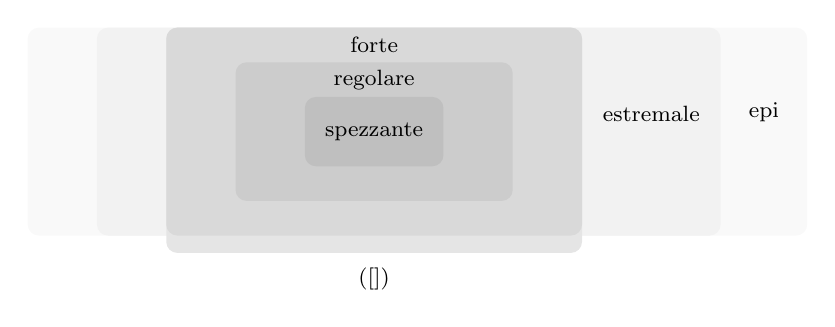
\begin{tikzpicture}[scale=1.1]
   % Outer to inner boxes
   \fill[gray!5,rounded corners] (-4,-1.2) rectangle (5,1.2);
   \node[font=\footnotesize,above] at (4.5,0.0) {epi};

   \fill[gray!10,rounded corners] (-3.2,-1.2) rectangle (4,1.2);
   \node[font=\footnotesize,above] at (3.2,0.0) {estremale};

   \fill[gray!20,rounded corners] (-2.4,-1.4) rectangle (2.4,1.2);
   \node[font=\footnotesize] at (0,-1.7) {$\lort(\Mono[\ctC])$};
   \fill[gray!30,rounded corners] (-2.4,-1.2) rectangle (2.4,1.2);
   \node[font=\footnotesize] at (0,1) {forte};

   \fill[gray!40,rounded corners] (-1.6,-0.8) rectangle (1.6,0.8);
   \node[font=\footnotesize] at (0,0.6) {regolare};

   \fill[gray!50,rounded corners] (-0.8,-0.4) rectangle (0.8,0.4);
   \node[font=\footnotesize] at (0,0) {spezzante};
  \end{tikzpicture}
 \end{center}
 \caption{Gerarchia delle classi di epimorfismi in una categoria \(\ctC\). Le inclusioni si possono invertire sotto le ipotesi indicate. Le classi \(\Epi[\ctC]^s\) degli epi forti di \ref{mepi_forte} e l'ortogonale sinistro \(\lort(\Mono[\ctC])\) sono `essenzialmente sempre' coincidenti nei casi reali, ma \ref{strepi_not_epi} è un controesempio. Ipotesi opportune su \(\ctC\) rovesciano alcune di queste inclusioni.}\label{fig_gerarchia}
\end{figure}
\subsection{Interazioni tra limiti e colimiti, completamenti}\index{Completamento!--- libero}
\subsubsection{Sulla commutatività dei limiti con i colimiti}\label{sec_comm_limcolim}

\begin{color}{blue}
 Questa parte dovrebbe essere la prosecuzione naturale della sezione precedente.
\end{color}

\begin{remark}\label{rem_noncomm_limcolim}
 È importante chiarire che, benché la proposizione \ref{prop_fubini} valga tanto per i limiti che (nella sua versione duale)
 per i colimiti, in generale i limiti non commutano con i colimiti. Precisiamo il problema: se \(G \colon \ctC \times \ctD \fun \ctB\)
 è un funtore, si ha effettivamente una freccia canonica \(\delta\) determinata dalla commutatività del seguente diagramma,
 dove le frecce senza nome sono le frecce canoniche del limite e del colimite
 \[\xymatrix{\colim_{\ctD}(\lim_{\ctC}G(C,D)) \ar[rr]^{\delta} & & \lim_{\ctC}(\colim_{\ctD}G(C,D)) \ar[d] \\
  \lim_{\ctC}G(C,D) \ar[u] \ar[r] & G(C,D) \ar[r] & \colim_{\ctD}G(C,D)}\]
 (ammesso evidentemente che tali limiti e colimiti esistano in \(\ctB\)), ma in generale tale freccia non è un isomorfismo,
 come mostra il seguente esempio.
\end{remark}

\begin{example}\label{ex_noncomm_limcolim}
 Prendiamo \(\ctC = \ctD = \{0,1\}\), la categoria discreta con due oggetti distinti, e \(G \colon \ctC \times \ctD \fun \ctSet\)
 il funtore costante che associa a ogni oggetto l'insieme 2 a due elementi. Il dominio e il codominio della freccia \(\delta\)
 in questo caso sono, rispettivamente, \((2 \times 2) + (2 \times 2)\) e \((2 + 2) \times (2 + 2)\). Per ovvie ragioni di cardinalità,
 non ci può essere nessuna biiezione fra tali insiemi.
\end{example}

Nei teoremi \ref{th_caratt_sifted} e \ref{th_caratt_filtr} espliciteremo due casi importanti in cui la freccia \(\delta\) dell'osservazione
\ref{rem_noncomm_limcolim} è un isomorfismo. Come risultato preliminare alla dimostrazione del teorema \ref{th_caratt_sifted}
ci occorre una caratterizzazione dei funtori iniziali in termini di colimiti. Ci limitiamo a dimostrare solo una delle due implicazioni
(quella che interviene nella prova del teorema), la seconda sarà proposta come esercizio. Ricordiamo che una categoria \(\ctD\) è
connessa se è non vuota e se per ogni coppia di oggetti \(X,Y \in \ctD\) esiste uno zig-zag di frecce che li connette
\[X \longleftarrow D_1 \longrightarrow D_2 \longleftarrow D_3 \longrightarrow D_4 \ldots\ldots D_{n-1} \longleftarrow D_n \longrightarrow Y\]
(vedi esercizio \ref{E.2.6.7}). Ricordiamo anche che un funtore \(F \colon \ctC \fun \ctD\) è iniziale se, per ogni oggetto \(D \in \ctD\), la
categoria comma \(D/F\) è connessa (vedi definizione \ref{2.8.61}).

\begin{lemma}\label{lemma_caract_funt_iniz}
 Un funtore \(F \colon \ctC \fun \ctD\) è iniziale se e solo se per ogni categoria \(\ctA\) e per ogni funtore \(G \colon \ctD \fun \ctA\),
 l'esistenza del colimite di \(G \cdot F\) implica che esiste il colimite di \(G\) e che la freccia canonica
 \[\beta \colon \colim_{\ctC}(G \cdot F) \to \colim_{\ctD}(G)\]
 è un isomorfismo.
\end{lemma}

\begin{proof} Precisiamo che \(\beta\) è l'unica freccia tale che il diagramma
 \[\xymatrix{\colim_{\ctC}(G \cdot F) \ar[rr]^-{\beta} & & \colim_{\ctD}(G) \\
  & G(FC) \ar[lu]^{\sigma_C} \ar[ru]_{s_{FC}} }\]
 commuta per ogni \(C \in \ctC\), dove le frecce \(\sigma_C\) e \(s_D\) sono le iniezioni nel colimite. \\
 \(\Rightarrow \colon\) Dobbiamo costruire il cocono colimite \(\{s_D \colon GD \to \colim_{\ctC}(G \cdot F)\}_{D \in \ctD}\).
 Per un oggetto \(D \in \ctD\) fissato, la categoria comma \(D/F\) è non vuota (perché connessa). Possiamo dunque scegliere
 una freccia \(u_D \colon D \to FX\) e porre
 \[s_D = \sigma_X \cdot G(u_D) \colon GD \to G(FX) \to \colim_{\ctC}(G \cdot F)\]
 Dobbiamo verificare che \(s_D\) è ben definita, cioè non dipende dalla scelta della freccia \(u_D\). Una volta fatto questo,
 la verifica che la famiglia \(\{s_D\}_{D \in \ctD}\) è naturale è simile (ma più semplice) e la verifica della proprietà universale
 è diretta (usando naturalmente la proprietà universale del colimite di \(G \cdot F\)). Supponiamo quindi di avere una seconda
 freccia \(v_D \colon D \to FY\). Poiché \(D/F\) è connessa, si può trovare uno zig-zag in \(D/F\) che connette \(u_D\) e \(v_D\)
 (per semplificare la scrittura dei diagrammi utilizzati nella dimostrazione, supponiamo che lo zig-zag sia ridotto a un'unica spanna,
 ma l'argomento è chiaramente generale), ovvero che si abbia un diagramma commutativo del tipo
 \[\xymatrix{ & D \ar[ld]_{u_D} \ar[d]^{f} \ar[rd]^{v_D} \\
  FX & FZ \ar[l]^-{Fx} \ar[r]_-{Fy} & FY}\]
 Applicando il funtore \(G\) a tale diagramma, si ottiene
 \[\xymatrix{ & &\colim_{\ctC}(G \cdot F) \\
  G(FX) \ar[rru]^{\sigma_X} & & & & GD  \ar[llll]_-{G(u_D)} \ar@{-->}[llu]_{s_D} \ar[llld]_>>>>>>>>>>>>>>>>>>>>{G(f)} \ar[ld]^{G(v_D)} \\
  & G(FZ) \ar[lu]^{G(Fx)} \ar[ruu]^>>>>>>>>>>{\sigma_Z} \ar[rr]_{G(Fy)} & & G(FY) \ar[luu]_>>>>>>>>>>{\sigma_Y} }\]
 Bisogna mostrare che \(\sigma_X \cdot G(u_D) = \sigma_Y \cdot G(v_D)\) usando la naturalità del cocono \(\{\sigma_C\}_{C \in \ctC} \colon\)
 \[\sigma_X \cdot G(u_D) = \sigma_X \cdot G(Fx) \cdot G(f) = \sigma_Z \cdot G(f) = \sigma_Y \cdot G(Fy) \cdot G(f) = \sigma_Y \cdot G(v_D)\]
 Consideriamo che questo sia sufficiente come dimostrazione della prima implicazione.
\end{proof}

Per la prova del teorema \ref{th_caratt_sifted} ci saranno utili 	anche i seguenti facili esercizi.

\begin{exercise}\label{exer_set_conn}
 Ogni categoria setacciata è connessa.
\end{exercise}

\begin{exercise}\label{exer_colim_cost}
 Sia \(F \colon \ctD \fun \ctB\) un funtore costante di valore \(X \in \ctB\). Se \(\ctD\) è connessa, allora il colimite di \(F\)
 è \(\{\id_X \colon F(D) = X \to X\}_{D \in \ctD}\). (Se \(X\) è l'oggetto iniziale di \(\ctB\), allora l'ipotesi che \(\ctD\) sia
 connessa è superflua.)
\end{exercise}

Enunciamo ora i due teoremi che caratterizzano le categorie setacciate e filtrate in termini di commutazione fra limiti e colimiti.
Per il momento ci limitiamo a dimostrare l'implicazione \(\Rightarrow\) del teorema \ref{th_caratt_sifted}, in quanto è quella
che serve nel capitolo \ref{cap_cat_alg}, dedicato alle categorie algebriche, per costruire certi colimiti. L'implicazione opposta e
la dimostrazione del teorema \ref{th_caratt_filtr} saranno proposte come esercizi.

\begin{theorem}\label{th_caratt_sifted}
 Una categoria piccola \(\ctD\) è setacciata (nel senso della definizione \ref{2.5.44}) se e solo se per ogni categoria discreta e
 finita \(\ctC\) e per ogni funtore \(G \colon \ctC \times \ctD \fun \ctSet\), la freccia canonica
 \[\delta \colon \colim_{\ctD}(\lim_{\ctC}G(C,D)) \to \lim_{\ctC}(\colim_{\ctD}G(C,D))\]
 è un isomorfismo.
\end{theorem}

\begin{proof} \(\Rightarrow \colon\) Assumiamo che la categoria \(\ctD\) sia setacciata e mostriamo che la freccia \(\delta\)
 dell'osservazione \ref{rem_noncomm_limcolim} è un isomorfismo. Poiché \(\ctC\) è finita e discreta, per induzione
 basta considerare due casi, il caso in  cui \(\ctC\) contiene solo due elementi distinti e il caso in  cui \(\ctC\) è vuota. \\
 Caso \(\ctC = \{1,2\} \colon\) in questa situazione dare un funtore \(G \colon \ctC \times \ctD \fun \ctSet\) significa scegliere due
 funtori \(H_1 = G(1,-), H_2 = G(2,-) \colon \ctD \fun \ctSet\). La freccia \(\delta\) è dunque
 \[\xymatrix{\colim_{\ctD}(H_1 \times H_2) \ar[rr]^-{\delta} & & \colim_{\ctD}(H_1) \times \colim_{\ctD}(H_2) \\
  & H_1(D) \times H_2(D) \ar[lu]^{\sigma_D} \ar[ru]_{s^1_D \times s^2_D} }\]
 dove \(H_1 \times H_2 \colon \ctD \fun \ctSet\) è il prodotto di \(H_1\) e \(H_2\) nella categoria \(\ctSet^{\ctD}\) (vedi proposizione
 \ref{prop_lim_puntuali}) e \(\{\sigma_D\}_{D \in \ctD}, \{s^1_D\}_{D \in \ctD}, \{s^2_D\}_{D \in \ctD}\) sono i coconi colimite.
 Osserviamo che
 \[\xymatrix{ & \ctD \times \ctD \ar[rd]^{H_1 \boxtimes H_2} \\
   \ctD \ar[ru]^{\Delta} \ar[rr]_{H_1 \times H_2} & & \ctSet }\]
 dove \(\Delta(D) = (D,D)\) e \(H_1 \boxtimes H_2)(D_1,D_2) = H_1(D_1) \times H_2(D_2)\) (questo è un caso particolarmente
 semplice dell'esercizio \ref{exer_lim_puntuali}). Poichè \(\ctD\) è setacciata, il funtore \(\Delta\) è iniziale (teorema \ref{2.8.65})
 e quindi, per il lemma \ref{lemma_caract_funt_iniz}, si ha un isomorfismo
 \[\beta \colon \colim_{\ctD}(H_1 \times H_2) = \colim_{\ctD}((H_1 \boxtimes H_2) \cdot \Delta) \to
  \colim_{\ctD \times \ctD}(H_1 \boxtimes H_2)\]
 Per mostrare che \(\delta = \beta\), e quindi che \(\delta\) è un isomorfismo, rimane da provare che
 \[\{s^1_{D_1} \times s^2_{D_2} \colon H_1(D_1) \times H_2(D_2) \to
  \colim_{\ctD}(H_1) \times \colim_{\ctD}(H_2)\}_{(D_1,D_2) \in \ctD \times \ctD}\]
 è il cocono colimite del funtore \(H_1 \boxtimes H_2\). Questa è una conseguenza del fatto che \(\ctSet\) è cartesiana chiusa
 (esempio \ref{ex_set_cartcl}). Esplicitamente, dato un cocono
 \[\{x_{D_1,D_2} \colon H_1(D_1) \times H_2(D_2) \to X\}_{(D_1,D_2) \in \ctD \times \ctD}\]
 l'unica fattorizzazione \(x \colon \colim_{\ctD}(H_1) \times \colim_{\ctD}(H_2) \to X\) delle frecce \(x_{D_1,D_2}\) attraverso le frecce
 \(s^1_{D_1} \times s^2_{D_2}\) si ottiene grazie alle seguenti biiezioni naturali fra l'insieme delle funzioni al di sopra della linea
 orizzontale e l'insieme delle funzioni al di sotto della linea:
 \[\begin{array}{c}
   x \colon \colim_{\ctD}(H_1) \times \colim_{\ctD}(H_2) \to X           \\ \hline
   \colim_{\ctD}(H_2) \to \ctSet(\colim_{\ctD}(H_1),X)                   \\ \hline
   \{H_2(D_2) \to \ctSet(\colim_{\ctD}(H_1),X)\}_{D_2 \in \ctD}          \\ \hline
   \{\colim_{\ctD}(H_1) \times H_2(D_2) \to X\}_{D_2 \in \ctD}           \\ \hline
   \{\colim_{\ctD}(H_1) \to \ctSet(H_2(D_2),X)\}_{D_2 \in \ctD}          \\ \hline
   \{\{H_1(D_1) \to \ctSet(H_2(D_2),X)\}_{D_1 \in \ctD}\}_{D_2 \in \ctD} \\ \hline
   \{\{x_{D_1,D_2} \colon H_1(D_1) \times H_2(D_2) \to X\}_{D_1 \in \ctD}\}_{D_2 \in \ctD}
  \end{array}\]
 Caso \(\ctC = \emptyset \colon\) in questa situazione la freccia \(\delta\) è la freccia terminale
 \[\delta \colon \colim_{\ctD}(T) \to \{\ast\}\]
 dove \(T \colon \ctD \fun \ctSet\) è l'oggetto terminale della categoria \(\ctSet^{\ctD}\), cioè il funtore costante definito
 da \(T(D) = \{\ast\}\). Poichè \(\ctD\) è setacciata, è anche connessa (esercizio \ref{exer_set_conn}) e quindi l'esercizio
 \ref{exer_colim_cost} permette di concludere che \(\delta\) è un isomorfismo.
\end{proof}

\begin{theorem}\label{th_caratt_filtr}
 Una categoria piccola \(\ctD\) è filtrata (nel senso della definizione \ref{2.5.41}) se e solo se per ogni categoria
 finite \(\ctC\) e per ogni funtore \(G \colon \ctC \times \ctD \fun \ctSet\), la freccia canonica
 \[\delta \colon \colim_{\ctD}(\lim_{\ctC}G(C,D)) \to \lim_{\ctC}(\colim_{\ctD}G(C,D))\]
 è un isomorfismo.
\end{theorem}

\begin{remark}\label{oss_unioni_filtr_sg}
 Per aiutare la lettrice a capire l'interesse dei teoremi \ref{th_caratt_sifted} e \ref{th_caratt_filtr} ricordiamo che, come già detto,
 nel capitolo \ref{cap_cat_alg} essi saranno utilizzati per mostrare che nelle categorie algebriche i colimiti setacciati si calcolano
 come colimiti degli insiemi soggiacenti (in un senso che verrà precisato), come è per altro il caso di tutti i limiti nelle categorie
 algebriche. Per vedere un esempio facile di tale situazione, si può pensare a una famiglia \(\{H_i\}_{i \in I}\) di sottogruppi di un
 gruppo \(G\), famiglia indicizzata da un insieme \(I\). L'intersezione insiemistica \(\bigcap_{i \in I}H_i\)  (che è un tipo di limite)
 è chiaramente un sottogruppo di \(G\). Invece l'unione \(\bigcup_{i \in I}H_i\) (che è un colimite) in generale non lo è.
 Se però l'insieme \(I\) è un insieme ordinato in cui ogni sottoinsieme finito ammette un maggiorante (e in particolare se è un
 insieme totalmente ordinato), ovvero se, visto come categoria, è filtrata, allora l'unione (che diventa in tal caso un colimite filtrato)
 è chiaramente un sottogruppo. Questa situazione, benché semplice, è di notevole importanza: si pensi alla dimostrazione
 del teorema di Krull (ogni ideale proprio di un anello commutativo è contenuto in un ideale massimale) o al fatto che in un
 anello noetheriano ogni catena ascendente di ideali si stabilizza.
\end{remark}


\begin{proposition}[Commutatività di colimiti filtrati e limiti finiti]\label{prop_commutativita_colimiti_filtrati_limiti_finiti}\index{Colimite!filtrato!commutatività con limiti finiti}\index{Limite!finito!commutatività con colimiti filtrati}
 \Todo{}
\end{proposition}

\begin{proposition}[Commutatività di colimiti setacciati e prodotti]\label{prop_commutativita_colimiti_setacciati_prodotti}\index{Colimite!--- setacciato}
 \Todo{}
\end{proposition}

\begin{definition}[Categoria di funtori polinomiali]\label{def_categoria_funtori_polinomiali}\index{Funtore!polinomiale}\index{Funtore!--- polinomiale}
 limiti e colimiti interagiscono per formare un polinomio
 \Todo{}
\end{definition}
\begin{example}\label{ex_colim_liste}\index{Liste!--- come colimite}
 \Todo{Liste come polinomi}
\end{example}
\begin{definition}[Completamento libero per diagrammi di forma \(\ctJ\)]\label{def_completamento_libero_diagrammi_ctJ}
 \Todo{}
\end{definition}

\Todo{Questa parte va riordinata secondo uno schema più razionale oppure rischia di diventare lunghissima e dispersiva; i completamenti liberi sono importanti, quindi vorrei dare: la definizione generale, l'esempio del completamento per coprodotti (e dualmente allora per prodotti) e il completamento di Cauchy; quindi copio `brutalmente' quello che ha scritto EnricoV e lo metteremo a posto}
\subsubsection{Completamento libero per prodotti}\label{sec_compl_somme_e_prod}
\Todo{}
\subsubsection{Completamento libero per idempotenti}\label{sec_compl_idemp}

\begin{color}{blue}
 Il completamento per idempotenti di una categoria è un argomento interessante che rientra nei teoremi di dualità
 per le teorie algebriche. Non so bene quale è il punto migliore del libro per introdurlo. Porta vari nomi: completamento per
 idempotenti, Cauchy completion, Karoubi envelope, \ldots Esito fra completamento per idempotenti e il più suggestivo
 completamento di Cauchy, che però, se adottato, richiede una spiegazione.
\end{color}

\hfill

Come secondo esempio di completamento, studiamo il completamento per idempotenti di una categoria.

\begin{definition}\label{def_idempotente}
 Una freccia \(f \colon X \to X\) di una categoria è detta idempotente se \(f \cmp f = f\).
\end{definition}

\begin{remark}\label{oss_idemp_eq}
 Dalla proposizione \ref{prop_equal_ass} sappiamo che, a partire da un diagramma commutativo del tipo
 seguente (che esprime il fatto che \(R\) è un  retratto di \(X\))
 \[ \xymatrix{R \ar[rr]^-{\id_R} \ar[rd]_{s} & & R \\ & X \ar[ru]_{r} } \]
 si ottengono un equalizzatore assoluto e un coequalizzatore assoluto nel modo seguente
 \[\xymatrix{R \ar[r]^-{s} & X \ar@<0.5ex>[r]^-{s \cmp r} \ar@<-0.5ex>[r]_-{\id_X} & X}
  \;\;\;\;\;\;\;\;\;\;\;\;
  \xymatrix{X \ar@<0.5ex>[r]^-{s \cmp r} \ar@<-0.5ex>[r]_-{\id_X} & X \ar[r]^-{r} & R}\]
 Osserviamo che la freccia \(s \cmp r \colon X \to X\) è idempootente, infatti \(s \cmp r \cmp s \cmp r = s \cmp \id \cmp r = s \cmp r\). \\
 Il prossimo lemma chiarisce il legame fra l'idempotenza della freccia \(s \cmp r\) e l'esistenza dell'equalizzatore e del coequalizzatore
 della coppia \((s \cmp r, \id_X)\).
\end{remark}

\begin{lemma}\label{lemma_spezz_idemp}
 Sia \(f \colon X \to X\) una freccia in una categoria \(\ctA\). Le condizioni seguenti sono equivalenti:
 \begin{enumerate}
  \item La freccia \(f\) si spezza: esistono \(s \colon R \to X\) ed \(r \colon X \to R\) tali che \(s \cmp r = f\) ed
        \(r \cmp s = \id_R\).
  \item La freccia \(f\) è idempotente ed esiste l'equalizzatore \(\xymatrix{R \ar[r]^-{s} & X \ar@<0.5ex>[r]^-{f} \ar@<-0.5ex>[r]_-{\id_X} & X}\)
  \item La freccia \(f\) è idempotente ed esiste il coequalizzatore \(\xymatrix{X \ar@<0.5ex>[r]^-{f} \ar@<-0.5ex>[r]_-{\id_X} & X \ar[r]^-{r} & R}\)
 \end{enumerate}
\end{lemma}

\begin{proof}
 \(1 \Rightarrow 2\) e \(1 \Rightarrow 3 \colon\) Questo è il contenuto della proposizione \ref{prop_equal_ass} e
 dell'osservazione \ref{oss_idemp_eq}. \\
 Ora mostriamo che \(2 \Rightarrow 1\), la prova dell'implicazione \(3 \Rightarrow 1\) è duale. Poiché \(f\) è
 idempotente, si ha \(f \cmp f = f = \id_X \cmp f\). La propriet\'a universale dell'equalizzatore fornisce un'unica freccia
 \(s \colon X \to R\) tale che \(s \cmp r = f\). Resta da mostrare che \(r \cmp s = \id_R\). Poiché \(s\) è un mono, tale
 uguaglianza si deduce dal fatto che \(s\) equalizza \(f\) e \(\id_X\), infatti \(s \cmp r \cmp s = f \cmp s = \id_X \cmp s = s \cmp \id_R\).
\end{proof}

\begin{definition}\label{def_idemp_compl}
 Una categoria è completa per idempotenti se tutte le sue frecce idempotenti si spezzano.
\end{definition}

\begin{remark}\label{oss_idCompl_retr}
 Segnaliamo qualche semplice conseguenza del lemma \ref{lemma_spezz_idemp}:
 \begin{enumerate}
  \item Una categoria che ha gli equalizzatori (o i coequalizzatori), è completa per idempotenti.
  \item Il fatto di essere completa per idempotenti è una condizione autoduale: una categoria \(\ctC\)
        è completa per idempotenti se e solo se \(\ctC^{\op}\) lo è.
  \item Una sottocategoria piena \(\ctB\) di una categoria \(\ctA\) completa per idempotenti è a sua
        volta completa per idempotenti se e solo se è chiusa in \(\ctA\) per retratti.
  \item Lo spezzamento di una freccia idempotente, quando esiste, è unico a meno di isomorfismi.
 \end{enumerate}
\end{remark}

Vediamo come si può costruire in modo universale una categoria completa per idemopotenti a partire da una categoria qualsiasi.

\begin{proposition}\label{prop_compl_idemp}
 Sia \(\ctC\) una categoria. Esistono una categoria completa per idempotenti \(\mathrm{Ic}(\ctC)\) e un funtore
 \(\mathrm{Ic}_{\ctC} \colon \ctC \fun \mathrm{Ic}(\ctC)\) tali che, per ogni categoria completa per idempotenti \(\ctB\) e per
 ogni funtore \(F \colon \ctC \fun \ctB\), esiste un funtore \(F' \colon \mathrm{Ic}(\ctC) \fun \ctB\) tale che il diagramma
 \[ \xymatrix{\ctC \ar[rr]^-{\mathrm{Ic}_{\ctC}} \ar[rd]_{F} & & \mathrm{Ic}(\ctC) \ar[ld]^{F'} \\ & \ctB }\]
 commuta a meno di un isomorfismo naturale. Inoltre, tale funtore \(F'\) è essenzialmente unico.
\end{proposition}

\begin{proof}
 Cominciamo col descrivere la categoria \(\mathrm{Ic}(\ctC)\).Un oggetto de \(\mathrm{Ic}(\ctC)\) è una freccia idempotente
 \(f \colon X \to X\) di \(\ctC\). Una freccia \(a \colon (f \colon X \to X) \to (g \colon Y \to Y)\) è una freccia \(a \colon X \to Y\) di
 \(\ctC\) tale che \(g \cmp a \cmp f = a\) o, equivalentemente, tale che \(a \cmp f = a\) e \(g \cmp a = a\)
 \[ \xymatrix{X \ar[r]^-{a} \ar[d]_{f} & Y \ar[d]^{g} \\
  X \ar[ru]^{a} \ar[r]_-{a} & Y }\]
 In effetti, se \(a \cmp f = f\) e \(g \cmp a = a\), allora \(g \cmp a \cmp f = g \cmp a = a\); viceversa, se \(g \cmp a \cmp f = a\),
 allora \(g \cmp a = g \cmp g \cmp a \cmp f = g \cmp a \cmp f = a\) e, analogamente, \(a \cmp f = a\). La composizione in
 \(\mathrm{Ic}(\ctC)\) è quella di \(\ctC\). La freccia identità in \(\mathrm{Ic}(\ctC)\) è
 \(f \colon (f \colon X \to X) \to (f \colon X \to X)\).
 Il funtore \(\mathrm{Ic}_{\ctC} \colon \ctC \fun \mathrm{Ic}(\ctC)\) è definito da
 \[ a \colon X \to Y \;\mapsto \; a \colon (\id_X \colon X \to X) \to (\id_Y \colon Y \to Y)\]
 Se \(h \colon (f \colon X \to X) \to (f \colon X \to X)\) è una freccia idempotente in \(\mathrm{Ic}(\ctC)\), il suo spezzamento è
 \[ (f \colon X \to X) \xto{h} (h \colon X \to X) \xto{h} (f \colon X \to X) \]
 Questo dimostra che \(\mathrm{Ic}(\ctC)\) è completa per idempotenti. \\
 Verifichiamo ora la proprietà universale. Se si applica la descrizione dello spezzamento di
 una freccia idempotente al caso dell'immagine in \(\mathrm{Ic}(\ctC)\) di una freccia idempotente \(f \colon X \to X\) di \(\ctC\),
 ne segue che, per ogni freccia \(a \colon (f \colon X \to X) \to (g \colon Y \to Y)\) di \(\mathrm{Ic}(\ctC)\), le due righe del
 diagramma commutativo
 \[ \xymatrix{(X \xto{f} X) \ar[rr]^-{f} \ar[d]_{a} & &
  \mathrm{Ic}_{\ctC}(X) \ar@<0.5ex>[rr]^-{\mathrm{Ic}_{\ctC}(f)} \ar@<-0.5ex>[rr]_-{\id} \ar[d]_{\mathrm{Ic}_{\ctC}(a)}
  & & \mathrm{Ic}_{\ctC}(X) \ar[d]^{\mathrm{Ic}_{\ctC}(a)} \\
  (Y \xto{g} Y) \ar[rr]_-{g} & & \mathrm{Ic}_{\ctC}(Y) \ar@<0.5ex>[rr]^-{\mathrm{Ic}_{\ctC}(g)} \ar@<-0.5ex>[rr]_-{\id}
  & & \mathrm{Ic}_{\ctC}(Y) }\]
 sono equalizzatori assoluti. Se ora abbiamo un funtore \(F \colon \ctC \fun \ctB\), l'unico modo di definire un funtore
 \(F' \colon \mathrm{Ic}(\ctC) \fun \ctB\) tale che \(F' \cmp \mathrm{Ic}_{\ctC} \simeq F\) è di definirlo come l'estensione
 agli equalizzatori nel diagramma seguente
 \[ \xymatrix{F'(f) \ar[r] \ar[d]_{F'(a)} & FX \ar@<0.5ex>[rr]^-{F(f)} \ar@<-0.5ex>[rr]_-{\id} \ar[d]_{F(a)} & & FX \ar[d]^{F(a)} \\
  F'(g) \ar[r] & FY \ar@<0.5ex>[rr]^-{F(g)} \ar@<-0.5ex>[rr]_-{\id} & & FY }\]
 Tale definizione è possibile perché \(\ctB\) è completa per idempotenti e le frecce \(F(f)\) e \(F(g)\) sono idempotenti.
\end{proof}

Per esprimere la proprietà universale \ref{prop_compl_idemp} in termini di un'equivalenza di categorie, utilizziamo un
lemma generale che richiede la nozione di suriettività a meno di retratti.

\begin{definition}\label{fef_sur_utr}
 Un funtore \(M \colon \ctC \fun \ctD\) è suriettivo a meno di retratti se ogni oggetto di \(\ctD\) è un retratto di un pggetto
 proveniente da \(\ctC\): per ogni \(D \in \ctD\) esiste un oggetto \(X \in \ctC\) e un diagramma del tipo
 \[\xymatrix{D \ar[rr]^-{\id_D} \ar[rd]_{s} & & D \\ & MX \ar[ru]_{r} }\]
\end{definition}

\begin{lemma}\label{lemma_indsur}
 Siano \(\ctB\) una categoria ed \(M\colon \ctC \fun \ctD\) un funtore. Consideriamo il funtore \(\ctB^M \colon \ctB^\ctD \fun \ctB^\ctC\)
 indotto per composizione con \(M\).
 \begin{enumerate}
  \item Se \(M\) è suriettivo a meno di retratti, allora \(\ctB^M\) è fedele.
  \item Se \(M\) è pieno e suriettivo a meno di retratti, allora \(\ctB^M\) è pieno e fedele.
 \end{enumerate}
\end{lemma}

\begin{proof}
 1. Consideriamo due trasformazioni naturali \(\beta,\gamma \colon A \nat B \colon \ctD \rightrightarrows \ctB\) e supponiamo
 che per ogni oggetto \(X \in \ctC\) si abbia \(\beta_{MX} = \gamma_{MX} \colon AMX \to BMX\). Per un oggetto \(D \in \ctD\),
 scegliamo una presentazione del tipo
 \[(X \in \ctC, s \colon D \to MX, r \colon MX \to D, r \cmp s = \id_D)\]
 La commutatività del diagramma seguente, dovuta alla naturalità di \(\beta\) e \(\gamma\), mostra che
 \(\beta_D = \gamma_D\), il che conclude la prova della fedeltà del funtore \(\ctB^M\)
 \[\xymatrix{AD \ar[r]^-{As} \ar[d]_{\beta_D} & AMX \ar[r]^-{Ar} \ar[d]_{\beta_{MX}} \ar[d]|{=} \ar[d]^{\gamma_{MX}} & AD \ar[d]^{\gamma_D} \\
  BD \ar[r]_-{Bs} & BMX \ar[r]_-{Br} & BD }\]
 2. Sia ora \(\alpha \colon A \cmp M \nat B \cdot M \colon \ctC \rightrightarrows \ctB\) una trasformazione naturale. Cerchiamo
 una trasformazione naturale \(\beta \colon A \nat B \colon \ctD \rightrightarrows \ctB\) tale che \(\ctB^M(\beta) = \alpha\).
 Per un oggetto \(D \in \ctD\), scegliamo una presentazione
 \[(X \in \ctC, s \colon D \to MX, r \colon MX \to D, r \cmp s = \id_D)\]
 e poniamo
 \[\beta_D \colon \xymatrix{AD \ar[r]^-{As} & AMX \ar[r]^-{\alpha_X} & BMX \ar[r]^-{Br} & BD}\]
 Cominciamo col mostrare il carattere naturale della famiglia \(\beta = \{\beta_D \colon AD \to BD \mid D \in \ctD\}\). Per questo, sia
 \(h \colon D \to E\) una freccia in \(\ctD\) e scegliamo una presentazione
 \[(Y \in \ctC, v \colon E \to MY, u \colon MY \to E, u \cmp v = \id_E)\]
 per l'oggetto \(E\). Otteniamo una freccia \(v \cmp h \cmp r \colon MX \to MY\) e, poiché \(M\) è pieno, esiste una freccia
 \(f \colon X \to Y\) tale che \(M(f) = v \cmp h \cmp r\). Ora possiamo considerare il diagramma seguente, la cui commutatività mostra
 il carattere naturale di \(\beta\):
 \[\xymatrix{AD \ar[r]^-{As} \ar[d]_{Ah} & AMX \ar[r]^-{\alpha_X} \ar[d]_{AMf} & BMX \ar[r]^-{Br} \ar[d]^{BMf} & BD \ar[d]^{Bh} \\
  AE \ar[r]_-{Av} & AMY \ar[r]_-{\alpha_Y} & BMY \ar[r]_-{Bu} & BE }\]
 Il quadrato centrale commuta per la naturalità di \(\alpha\), il quadrato a destra commuta perché \(u
 \cmp M(f) = u \cmp v \cmp h \cmp r = h \cmp r\) e il quadrato di sinistra commuta perché \(M(f) \cmp s = v \cmp h \cmp r \cmp s = v \cmp h\).
 Se ora scegliamo \(E=D\) e \(h=\id_D\), lo stesso argomento mostra che \(\beta\) è ben definiuta, cioè \(\beta_D\) non dipende
 dalla presentazione scelta per \(D\). In particolrae, se \(D=MX\), come prsentazione possiamo scegliere
 \[(X \in \ctC, \id_{MX} \colon MX \to MX, \id_{MX} \colon MX \to MX)\]
 e otteniamo che \(\beta_{MX} = \alpha_X\), cioè che \(\ctB^M(\beta)=\alpha\).
\end{proof}

\begin{corollary}\label{cor_equiv_idcompl}
 Consideriamo due categorie \(\ctB\) e \(\ctC\), con \(\ctB\) completa per idempotenti. Il funtore
 \(\mathrm{Ic}_\ctC \colon \ctC \fun \mathrm{Ic}(\ctC)\) induce un'equivalenza
 \(\ctB^{\mathrm{Ic}_{\ctC}} \colon \ctB^{\mathrm{Ic}(\ctC)} \fun \ctB^\ctC\).
\end{corollary}

\begin{proof}
 Il funtore \(\mathrm{Ic}_{\ctC}\) è chiaramente pieno. Inoltre è anche suriettivo a meno di retratti perché il diagramma
 \[ \xymatrix{ (X \xto{f} X) \ar[r]^-{f} & \mathrm{Ic}_{\ctC}(X) \ar[r]^-{f} & (X \xto{f} X) }\]
 mostra che ogni oggetto di \(\mathrm{Ic}(\ctC)\) è un retratto di un oggetto proveniente da \(\ctC\). Qunidi il lemma
 \ref{lemma_indsur} garantisce che \(\ctB^{\mathrm{Ic}_{\ctC}}\) è pieno e fedele. Il carattere essenzialmente suriettivo di
 \(\ctB^{\mathrm{Ic}_{\ctC}}\) segue immediatamente dalla proprietà universale \ref{prop_compl_idemp}.
\end{proof}

Nel caso in cui la categoria \(\ctC\) sia piccola, ci tornerà utile più tardi una descrizione alternativa del completamento
per idempotenti (corollario \ref{cor_idcompl_ap}). Per preparare tale descrizione, e per completare il corollario
\ref{cor_equiv_idcompl}, analizziamo la proprietà universale di \(\mathrm{Ic}_{\ctC} \colon \ctC \fun \mathrm{Ic}(\ctC)\).

\begin{lemma}\label{lemma_caratt_idcompl}
 Siano \(\ctC\) e \(\ctD\) due categorie, con \(\ctD\) completa per idempotenti.
 Consideriamo la situazione della proposizione \ref{prop_compl_idemp}
 \[ \xymatrix{\ctC \ar[rr]^-{\mathrm{Ic}_{\ctC}} \ar[rd]_{M} & & \mathrm{Ic}(\ctC) \ar[ld]^{M'} \\ & \ctD }\]
 \begin{enumerate}
  \item Il funtore \(M'\) è un'equivalenza se e solo se \(M\) è pieno, fedele e suriettivo a meno di retratti.
  \item In particolare, \(\ctC\) è completa per idempotenti se e solo se \(\mathrm{Ic}_{\ctC}\) è un'equivalenza.
 \end{enumerate}
\end{lemma}

\begin{proof}
 1. Il funtore \(\mathrm{Ic}_{\ctC}\) è pieno, fedele e suriettivo a meno di retratti, come spiegato nella dimostrazione
 del corollario  \ref{cor_equiv_idcompl}. \\
 Viceversa, le frecce \((f \colon X \to X) \to (g \colon Y \to Y)\) di \(\mathrm{Ic}(\ctC)\) si riconducono a frecce del tipo
 \((f \colon X \to X) \to \mathrm{Ic}_{\ctC}(Y)\) perché \((g \colon Y \to Y)\) è un limite di oggetti provenienti da \(\ctC\). Inoltre,
 le frecce del tipo \((f \colon X \to X) \to \mathrm{Ic}_{\ctC}(Y)\) si riconducono a loro volta a frecce del tipo
 \(\mathrm{Ic}_{\ctC}(X) \to \mathrm{Ic}_{\ctC}(Y)\) perché \((f \colon X \to X)\) è un colimite di oggetti provenienti da \(\ctC\).
 Ma l'azione di \(M'\) su una freccia del tipo \(\mathrm{Ic}_{\ctC}(X) \to \mathrm{Ic}_{\ctC}(Y)\) coincide con l'azione di \(M\)
 sulla corrispondente freccia \(X \to Y\) e quindi \(M'\) è pieno e fedele se \(M\) lo è. Sia ora \(D \in \ctD\). Per ipotesi,
 esistono un oggetto \(X \in \ctC\) e due frecce \(s \colon D \to MX\) e \(r \colon MX \to D\) tali che \(r \cmp s = \id_D\). Poiché
 \(M\) è pieno, esiste una freccia \(f \colon X \to X\) tale che \(M(f) = s \cmp r\). Inoltre, tale freccia \(f\) è idempotente perché
 \(M(f)\) lo è e \(M\) è fedele. Finalmente, \(M'(f)\) è per definizione lo spezzamento di \(M(f)\) in \(\ctD\) e quindi è isomorfo
 a \(D\) perché lo spezzamento è essenzialmente unico. \\
 2. Se \(\mathrm{Ic}_{\ctC}\) è un'equivalenza, allora \(\ctC\) è completa per idempotenti perché \(\mathrm{Ic}(\ctC)\) lo è.
 Viceversa, se \(\ctC\) è completa per idempotenti, si può applicare il punto precedente prendendo come funtore \(F\) il funtore
 identico su \(\ctC\) e si ottiene che \(\mathrm{Ic}_{\ctC}\) è un'equivalenza.
\end{proof}

\begin{corollary}\label{cor_equiv_sutr}
 Consideriamo tre categorie \(\ctB, \ctC\) e \(\ctD\), con \(\ctB\) e \(\ctD\) complete per idempotenti, e un funtore \(M \colon \ctC \fun \ctD\).
 Se \(M\) è pieno, fedele e suriettivo a meno di retratti, allora il funtore indotto \(\ctB^M \colon \ctB^\ctD \fun \ctB^\ctC\) è
 un'equivalenza.
\end{corollary}

\begin{proof}
 Dalla decomposizione \(M = M' \cmp \mathrm{Ic}_\ctC\) della proposizione \ref{prop_compl_idemp} segue che
 \(\ctB^M = \ctB^{M' \cmp \mathrm{Ic}_{\ctC}} = \ctB^{\mathrm{Ic}_{\ctC}} \cmp \ctB^{M'}\). Poiché \(\ctB^{\mathrm{Ic}_{\ctC}}\)
 è un'equivalenza (corollario \ref{cor_equiv_idcompl}) e \(\ctB^{M'}\) è un'equivalenza (lemma \ref{lemma_caratt_idcompl}),
 anche \(\ctB^M\) è un'equivalenza.
\end{proof}

\begin{remark}\label{oss_idcompl_duale}
 Poiché il fatto di essere completa per idempotenti è una condizione autoduale, possiamo applicare il lemma
 \ref{lemma_caratt_idcompl} alla configurazione
 \[ \xymatrix{\ctC^{\op} \ar[rr]^-{\mathrm{Ic}_{\ctC^{\op}}} \ar[rd]_{M=\mathrm{Ic}_{\ctC}^{\op}} & & \mathrm{Ic}(\ctC^{\op}) \ar[ld]^{M'} \\
  & \mathrm{Ic}(\ctC)^{\op} }\]
 e il funtore \(M'\) che si ottiene fornisce un'equvalenza \(\mathrm{Ic}(\ctC^{\op}) \simeq \mathrm{Ic}(\ctC)^{\op}\).
\end{remark}

\begin{theorem}[Complemento]\label{mk_kelly_closure}
 Kelly closure of a class of colimits
 \cite{paper_kelly_closure}
 \Todo{}
\end{theorem}
